\documentclass[a4paper]{report}

% \usepackage[utf8]{inputenc}
% \usepackage[T1]{fontenc}
% \usepackage{textcomp}
\usepackage[english]{babel}
\usepackage{amsmath, amssymb}
\usepackage[separate-uncertainty=true, multi-part-units=single]{siunitx}
\usepackage[]{subfig}
\usepackage[colorlinks=true, anchorcolor=blue, linkcolor=blue, citecolor=blue, bookmarks=false,hyperfootnotes=false]{hyperref}
\usepackage[margin=1in]{geometry}
\usepackage{color,soul}
\usepackage{tabularx}


% figure support
\usepackage{import}
\usepackage{xifthen}
\pdfminorversion=7
\usepackage{pdfpages}
\usepackage{transparent}
\usepackage{physics}
\graphicspath{ {./figures/} }
% \setlength{\parindent}{0pt}
\usepackage{chngcntr}
\usepackage{verbatim}
\usepackage{indentfirst}
\usepackage[most]{tcolorbox}

\numberwithin{equation}{section}
\counterwithin{figure}{section}
\newcommand{\incfig}[1]{%
		\def\svgwidth{\columnwidth}
		\import{./figures/}{#1.pdf_tex}

}

\pdfsuppresswarningpagegroup=1

% for citations / references
\usepackage[style=ieee]{biblatex}
\addbibresource{styx-report.bib}

\begin{document}

%----------------------------------------------------------------------------------------
%	TITLE PAGE
%----------------------------------------------------------------------------------------
\begin{titlepage} % Suppresses displaying the page number on the title page and the subsequent page counts as page 1
	\newcommand{\HRule}{\rule{\linewidth}{0.5mm}} % Defines a new command for horizontal lines, change thickness here
	
	\center % Centre everything on the page
	%------------------------------------------------
	%	Headings
	%------------------------------------------------
	
	\textsc{\LARGE Rheinische Friedrich-Wilhelms-Universit\"at Bonn }\\[4cm] % Main heading such as the name of your university/college
	
	\textsc{\Large Advanced Laboratory Course}\\[0.5cm] % Major heading such as course name
	
	\textsc{\large Performed on: May 12 - 13, 2022}\\[0.5cm] % Minor heading such as course title

	\textsc{\large Submitted on: June 20, 2022}\\[0.5cm] % Minor heading such as course title
	
	%------------------------------------------------
	%	Title
	%------------------------------------------------
	
	\HRule\\[0.4cm]
	
	{\huge\bfseries E217: STYX}\\[0.4cm] % Title of your document
	
	\HRule\\[1.5cm]
	
	%------------------------------------------------
	%	Author(s)
	%------------------------------------------------
	
	\begin{minipage}{0.4\textwidth}
		\begin{flushleft}
			\large
			\textit{Authors}\\
			Keito Watanabe \\
			Paarth Thakkar
		\end{flushleft}
	\end{minipage}
	~
	\begin{minipage}{0.4\textwidth}
		\begin{flushright}
			\large
			\textit{Tutor(s)}\\
			Patrick Bauer
		\end{flushright}
	\end{minipage}

	\vspace*{5em}

	\begin{minipage}{0.8\textwidth}
		\begin{centering}
			% \large
			\textbf{Abstract}\\[0.2cm]
            
		\end{centering}
	\end{minipage}
	
	% If you don't want a supervisor, uncomment the two lines below and comment the code above
	%{\large\textit{Author}}\\
	%John \textsc{Smith} % Your name
	
	%------------------------------------------------
	%	Date
	%------------------------------------------------
	
	%\vfill\vfill\vfill % Position the date 3/4 down the remaining page
	% \vfill\vfill
	
	% {\large\today} % Date, change the \today to a set date if you want to be precise
	
	%------------------------------------------------
	%	Logo
	%------------------------------------------------
	
	%\vfill\vfill
	%\includegraphics[width=0.2\textwidth]{placeholder.jpg}\\[1cm] % Include a department/university logo - this will require the graphicx package
	 
	%----------------------------------------------------------------------------------------
	
	% \vfill % Push the date up 1/4 of the remaining page
	
\end{titlepage}



\tableofcontents

\chapter{Introduction} \label{chap:intro}

In this experiment, The Straw Tube Young student eXperiment (STYX), we study detect and study the secondary cosmic rays that reach the surface of earth. Elements of the experiment were originally part of ZEUS detector at DESY. 

The experiment starts off with getting familiar with the setup. This is followed by calibrating the detector to appropriate voltages so as to reduce noise and maximize the number of events. In the process, we also learn how to operate software tools such as the various classes of \texttt{Styx} and ROOT, an data analysis software developed by CERN. After the voltages have been set, the detector is left overnight to collect data. The next day, before starting the analysis, the data is further calibrated using straw-by-straw calibration. Then, the data is analyzed and various aspects of secondary cosmic rays are studied. 

In Chapter \ref{chap:theory}, we discuss the theoretical background behind necessary to gain insight about the experiment and it's setup. More specifically, we look at cosmic rays and various kinds of detectors used to study charged particles. In Chapter \ref{chap:exp_setup}, the experimental setup with each of it's components is discussed. In Chapter \ref{chap:procedure}, we look at how we go about setting the appropriate operating and threshold voltages for PhotoMultiplier Tubes (PMTs) and the Front-End (FE) electronics. In Chapter \ref{chap:calib}, we look at how the calibration process, straw-by-straw calibration is applied to the data. In Chapter \ref{chap:track_analysis}, having applied the calibration, we look at several properties of cosmic rays, more specifically, the muons. Lastly, we include additional plots and figures in the Appendix \ref{chap:appendix}. This report, closely follows the STYX lab manual \cite{labman}.

\chapter{Theory} \label{chap:theory}

\section{Cosmic Rays}



Primary cosmic rays are highly energetic charged particles or nuclei with a long lifetime of order $10^6$ years or longer that are accelerated by 
astrophysical origins. These particles mainly consist of protons (85\%), but also consist of heavier nuclei such as Helium \cite{Tanabashi2018}. 
These cosmic rays propagate through intergalactic and interstellar space, losing energy through radiative processes \cite{DeDomenico2012}.
They are then captured by the Earth's magnetic field before arriving at Earth's atmosphere with energies in MeV to GeV ranges. 
They then interact with the atmospheric nuclei on Earth, producing "secondaries", that is, particles produced from such interactions. The secondaries
produced are mainly pions ($\pi^\pm, \pi^0$), whereas kaons ($K^\pm, K^0, \bar{K}^0$) are only produced with a probability of 10\% compared to pions \cite{Grupen2005}. \par 

\begin{figure*}[!h]
	\centering
	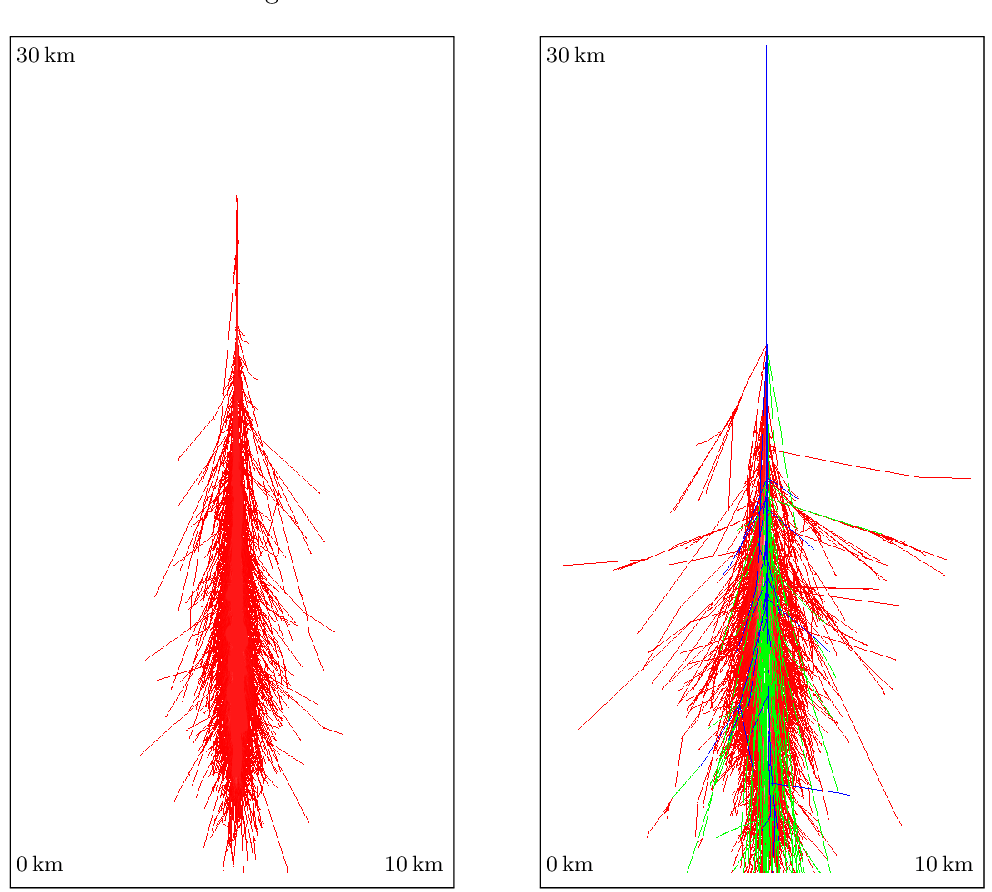
\includegraphics[width=0.6\textwidth]{em_hadronic_showers.png}
	\caption{ \textit{Left:} An electromagnetic shower induced by $\gamma$ at $\SI{1}{\tera\electronvolt}$. 
				\textit{Right: } A hadronic shower induced by a $\SI{1}{\tera\electronvolt}$ proton. Both plots show the lateral
				development of the showers at different altitudes. The red lines indicate electromagnetic components, blue indicates 
				hadronic components, and green indicate muon components (consisting of $\mu, \nu_\mu$). Obtained from Ref. \cite{Haeffner2014}. }
	\label{fig:em_had_showers}
\end{figure*}

As pions and kaons are not stable, they decay into subsequent particles through various channels.  
The neutral pion most commonly decay into a pair of photons ($\pi^0 \rightarrow \gamma + \gamma$), which subsequently produces a pair of electron and positron (pair production). They then undergo 
subsequent annihilation and bremsstrahlung processes, creating an electromagnetic cascade consisting of these three particles. Charged 
pions and kaons, however, primarily decay into a pair of muon and its corresponding neutrino or anti-neutrino ($\pi^+, K^+ \rightarrow \mu^+ + \nu_\mu$, $\pi^-, 
K^- \rightarrow \mu^- + \bar{\nu}_\mu$). These muons can also decay weakly into electrons, which then create subsequent electromagnetic cascades.
At higher energies of $E > \SI{10}{\giga\electronvolt}$, these pions and kaons can also decay into subsequent pions, which 
creates a hadronic cascade primarily consisting of these particles. Fig. \ref{fig:em_had_showers} shows an example of an electromagnetic and hadronic cascade that occurs from cosmic rays.


Through such electromagnetic and hadronic cascades, most charged particles are absorbed by the atmosphere and thus do not reach sea level. However, most of the muons 
produced from pions and kaons reach sea level due to their long lifetime, and as such approximately 80\% of the charged particles that reach sea level are muons.
The flux of muons detected at sea level is approximately 1 particle per cm$^2$ per minute, and as such one can detect more than $7 \times 10^{6}$ muons for an 
overnight measurement with a detector with an area of $\SI{1}{\meter\squared}$.  Neutrinos also reach sea level as they only interact weakly with matter and has a 
low interaction probability \cite{Grupen2005}. In the setup of our experiment, however, we are not able to detect neutrinos and thus only muons are detected. 
Fig. \ref{fig:air_shower} shows the schematic of a typical air shower from a primary cosmic ray. \par 


\begin{figure*}[!h]
	\centering
	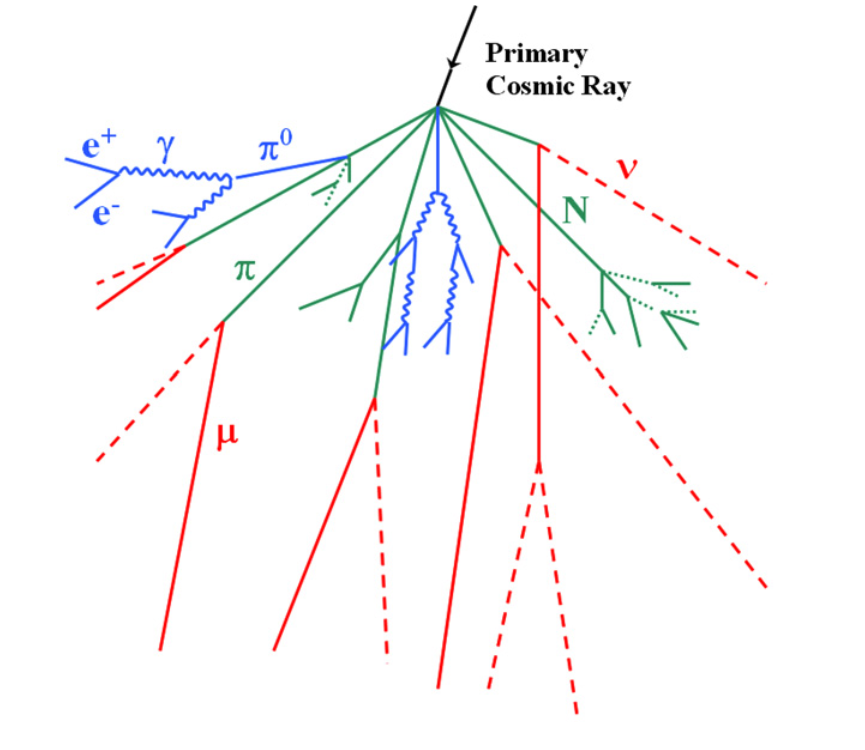
\includegraphics[width=0.6\textwidth]{air_shower.png}
	\caption{A typical air shower resulting from interaction of primary cosmic ray with the atmosphere. Electromagnetic cascades are shown in blue and hadronic 
	cascades are shown in green. The muons and neutrinos (indicated in red) produced from pion and kaon decays are the most common particles that reach sea level.
	Obtained from Ref. \cite{Blanco2009}.}
	\label{fig:air_shower}	
\end{figure*}

The total muon intensity distribution depends on the zenith angle $\theta$, i.e. the angle from the local zenith of the location of 
measurement. Such dependence is due to the stronger absorption of muons as they have to propagate through larger distances at 
inclined angles. The intensity distribution is given as such: 
\begin{equation}
    I(\theta) = I_0 \cos^n \theta 
	\label{eq:muon_intensity}
\end{equation}
where $I_0$ is the intensity at the local zenith ($\theta = 0^\circ$) \cite{Grupen2005}. The exponent of the cosine function at 
sea level is $n = 2$ as most muons have energies $E_\mu \sim \SI{3}{\giga\electronvolt}$ when they reach sea level \cite{Stefano2012}.

\section{Gaseous Detectors}

To detect the muons that originate from cosmic ray showers, we use ionization detectors which collects the ionized electrons and ions 
from the emitted radiation from such muons. The basic configuration of an gaseous ionization detector is 
made of a cylindrical container with conducting walls, representing the cathode, that is filled with a noble gas such as argon. A positive voltage 
$+V_0$ is applied through a conducting wire, representing the anode, which is then connected to the thin end window.
See Fig. \ref{fig:ionization_chamber_schematic} 
for a schematic of the ionization detector with this setup. From this, a radial electric field of the following form is generated within the chamber:
\begin{equation}
	E(r) = \frac{1}{r}\frac{V_0}{\ln (b / a)}
\end{equation}
where $r$ is the radial distance from the axis, $b$ is the inner radius of the cylinder, and $a$ is the outer radius of the conducting 
wire as shown in Fig. \ref{fig:ionization_chamber_schematic}. \par 

\begin{figure*}[!h]
	\centering
	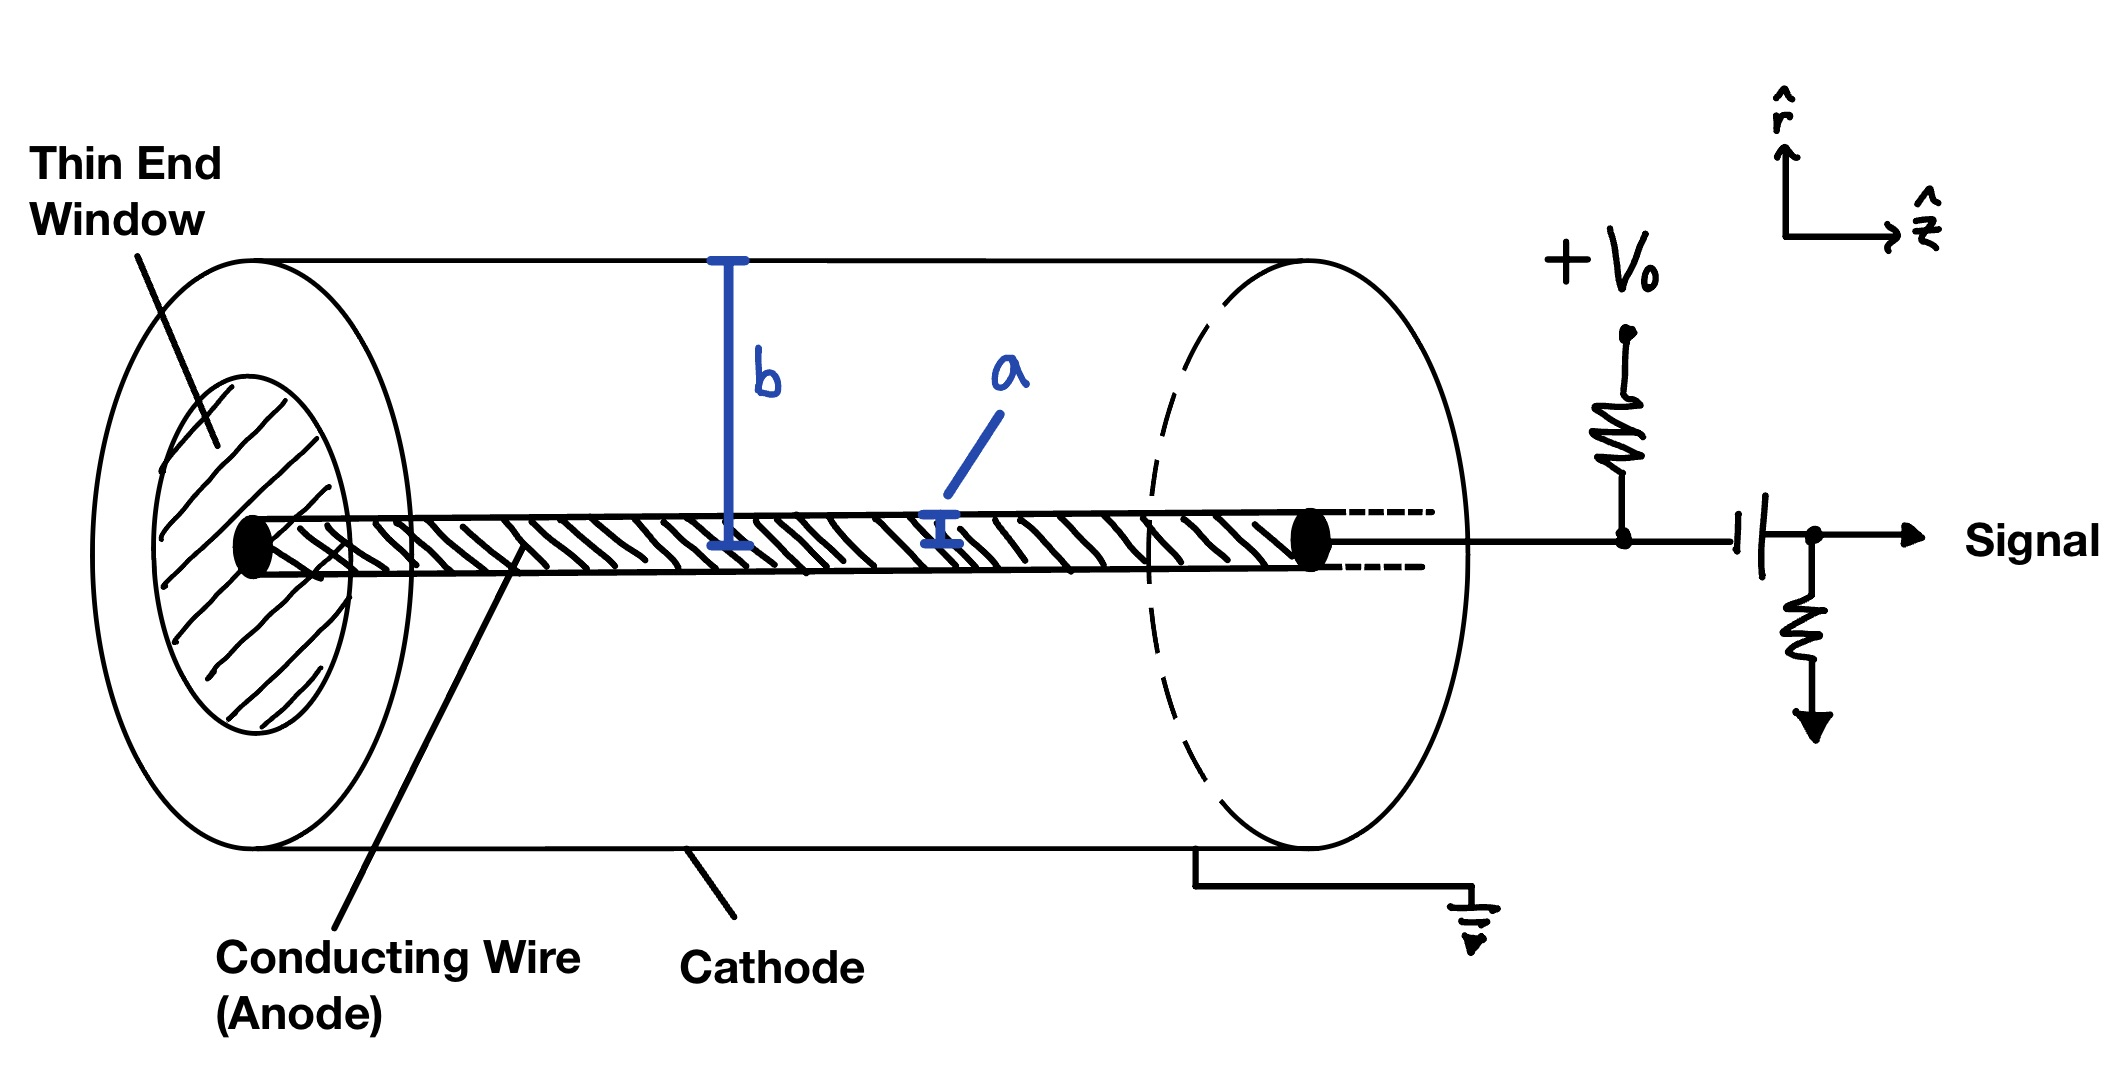
\includegraphics[width=0.6\textwidth]{ionization_chamber_schematic.png}
	\caption{Schematic of an gaseous ionization detector based on Ref. \cite{Leo1994}. Here, $b$ is the inner radius of the cylinder (cathode) and $a$ is the outer radius 
	of the conducting wire (anode).}
	\label{fig:ionization_chamber_schematic}	
\end{figure*}

As such, as the charged particles traverses through the detector it produces electron-ion pairs. Due to the resulting electric field, 
the electrons and ions drift towards the anode and cathode respectively. The signal from the anode can then be used for detection of the 
traversing charged particle \cite{Leo1994}. \par 

The signal obtained from the ionization detector depends on the field intensity and thus the applied voltage $V_0$. Fig. \ref{fig:ionization_regions} shows the 
dependency of the number of ions collected with the applied voltage for two types of incident particles. This dependence can be separated into six regions:
\begin{enumerate}
	\item \textbf{Recombination Region}: For low voltages, the electric field is not strong enough to accelerate the electron-ion pairs, thus allowing them to recombine 
			before they are collected.
	\item \textbf{Ionization Region}: At some voltage, enough voltage is applied so that all electron and ions are collected in their respective electrodes. 
			A plateau is observed in this region as increasing the voltage will not affect the number of ions or electrons collected. Ionization chambers operate in this region.
	\item \textbf{Region of Proportionality}: If we increase the voltage past the plateau region, the electric field is strong enough to accelerate the electrons to ionize the gas molecules 
			in the cylinder. Electrons produced from the ionization will further ionize other gas molecules, creating an ionization avalanche or cascade. As $E \propto r^{-1}$,
			the electric field is strongest near the anode so the avalanche occurs very quickly before electrons are collected by the anode. Since the number of electron-ion
			pairs are directly proportional to the number of primary electrons, the number of ions collected is proportional to the applied voltage $V_0$. Proportionality
			chambers are operated within this region, and is the most relevant region for our experiment.
	\item \textbf{Region of Limited Proportionality}: As we increase the voltage further, the proportionality is lost as the space charges distorts the electric field
			near the anode. 
	\item \textbf{Saturation Region}: Further increasing the voltage, the increased energy causes discharge within the gas. A chain reaction of avalanches occur 
			throughout the anode, causing the output signal to be saturated. The amplitude of the signal will remain the same even when increasing the energy, 
			yielding the second plateau. To prevent this effect, a quenching gas is often placed in the medium to absorb the photons causing the chain reaction. 
			Geiger-M{\"u}ller counters operate in this region.
	\item \textbf{Discharge Region}: Above the saturation region, continous discharge occurs throughout the cylinder which can damage the detector. As such, this region
			is to be avoided when operating the detector.
\end{enumerate}

\begin{figure*}[!h]
	\centering
	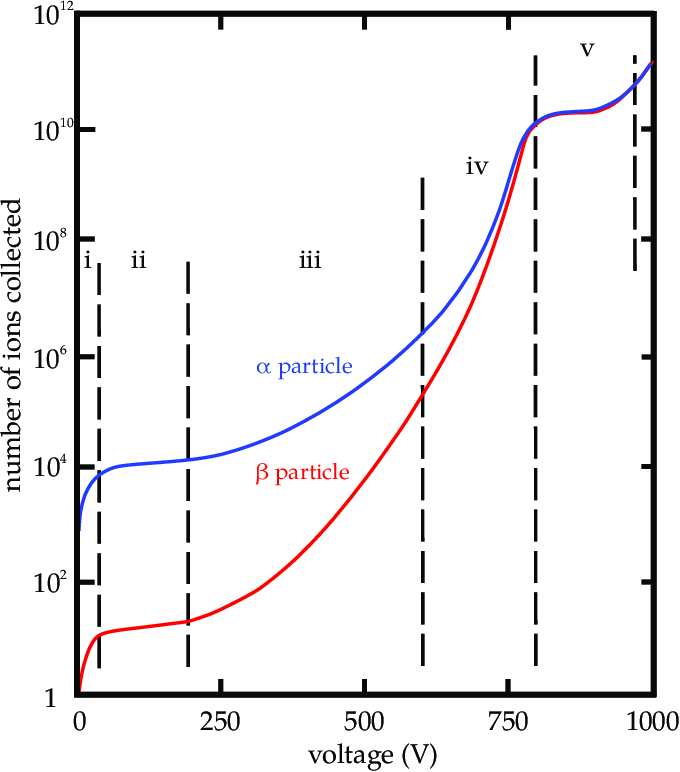
\includegraphics[width=0.5\textwidth]{ionization_regions.png}
	\caption{Number of ions collected at different applied voltage where the incident particles are $\alpha$ or $\beta$ particles. 
	The first five regions as mentioned in the script are labelled (i) - (v) in the plot, and the sixth region can be seen to the right of region (v). 
	Obtained from Ref. \cite{Lukas2018}. }
	\label{fig:ionization_regions}	
\end{figure*}

\section{Drift Chambers}

In our experiment, we use a type of proportional chamber called a drift chamber, also known as "straws". The drift chamber allows one to determine the spatial information 
of the traversing particle by measuring the drift time of the ionized electrons. The position of the produced electrons from the anode wire is 
given as such: 
\begin{equation}
	x = \int_{t_0}^{t_1} u dt
\end{equation}
where $t_0$ is the arrival time of the particle, $t_1$ is the time in which the signal reaches the anode, and $u$ is the drift velocity. To obtain a 
linear depedence with time and distance, a constant drift velocity and thus a constant electric field is desired. Using drift chambers, one can 
construct a constant electric field. \par 

\begin{figure*}[!hb]
	\centering
	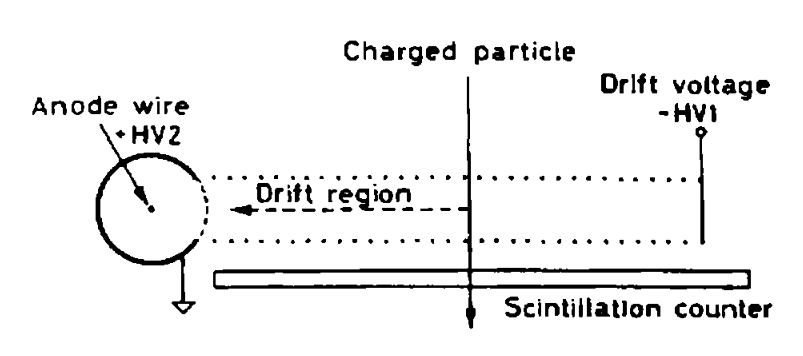
\includegraphics[width=0.6\textwidth]{drift_chamber.png}
	\caption{Schematic of a typical drift chamber. The scintillator counter is placed below the chamber. The 
	traversing charged particle ionizes the gas molecules, and the electrons drift with a constant drift velocity (due to the 
	applied drift voltage) towards the 
	anode, where the signal is created. Obtained from Ref. \cite{Leo1994}.}
	\label{fig:drift_chamber}	
\end{figure*}


The drift chamber is constructed by placing a series of cathode field wires at appropriate voltages in between a high voltage electrode and 
an anode of a simple proportional counter. A scintillation counter is placed before or after the chamber to signal the arrival of a particle. Refer to 
Sec.  \ref{sec:scint_pmt} for more details about the scintillator counter. 
Once the charged particles passes through the chamber and scintillator, the liberated electrons drift to the anode. The fast signal from the scintillator
starts a timer at the same time. The timer is then stopped from the signal created at the anode by the drifting electrons. See Fig. \ref{fig:drift_chamber} for a schematic of a typical 
drift chamber \cite{Leo1994}. In our experiment, we use multiple straws with several layers to more accurately determine the position of the 
atmospheric muons. \par 

\section{Scintillation Detectors and Photomultiplier Tubes} \label{sec:scint_pmt}

Certain materials emit a small flash of light, i.e. a scintillation, when they are struck by nuclear particles or radiation.
With an amplifying device such as a photomultiplier tube (PMT), one can convert the scintillation into an electric pulse
using a scintillation detector. The electric pulse is then analyzed to study about the incident radiation. Scintillation detectors 
are useful especially due to their high sensitivity to energy measurements, their fast time response, and their ability 
to discriminate between pulse shapes. \par 

A scintillator detector is constructed from a scintillating materia which is optically coupled to a PMT. The radiation excites the 
atom or molecule in the scintillating material, causing scintillation to occur. The PMT then converts and amplifies the light into 
an electric current which is then read out by an electronics system \cite{Leo1994}. The scintillation detectors used in our experiment 
operate under the same principles as above. \par 


The photomultiplier tubes used within the scintillation detectors convert detected photons into electronic current that can 
be measured. The photons are collected from a photocathode before emitting an electron due to the photoelectric effect. The electrons 
are then multiplied by a series of dynodes which emits secondary electrons within the material due to transfer of energy. An applied 
voltage is also applied in this region to accelerate these electrons, subsequently producing more electrons. The constructed cascade is 
collected at the anode to give a measurable electronic current \cite{Leo1994}. Fig. \ref{fig:pmt_schematic} shows the schematic of a typical photomultiplier tube. 


\begin{figure*}[!h]
	\centering
	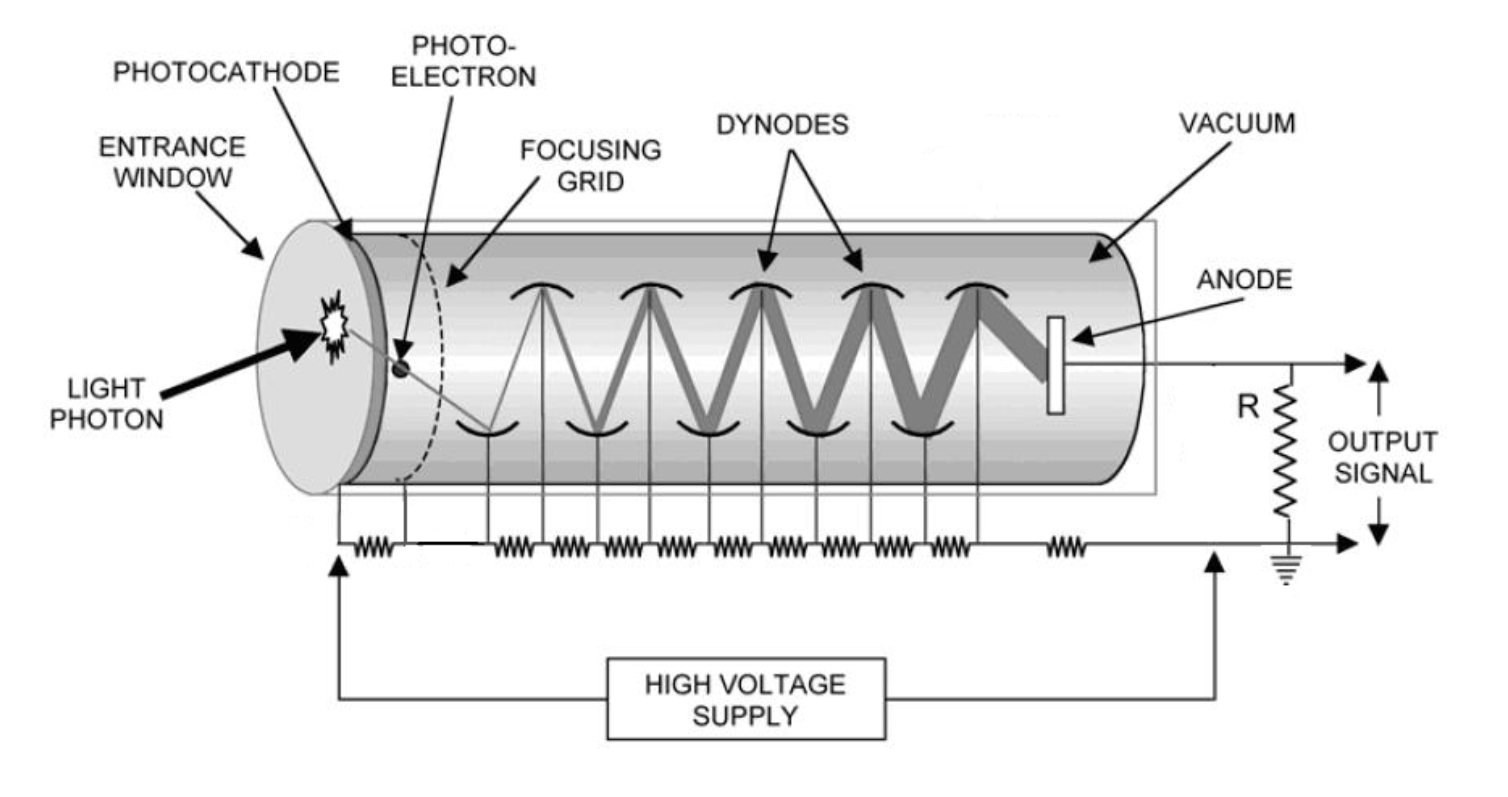
\includegraphics[width=0.6\textwidth]{pmt_schematic.png}
	\caption{Schematic of a typical photomultiplier tube. Photons are detected at the cathode, before entering the focusing grid,
	 and the electrons are accelerated by the multiple dynodes before collected at the anode to produce an electronic signal.
	 Obtained from Ref. \cite{Danisch2014}.}
	\label{fig:pmt_schematic}	
\end{figure*}


\chapter{Experimental Setup} \label{chap:exp_setup}

\section{Detectors}

The experimental setup is shown in Fig. \ref{fig:setup1}. The setup consists of two major components, the modules, which are the three copper-colored trapezoids, and the trigger system, which are the two black panels. 

\begin{figure}[htpb]
    \centering
    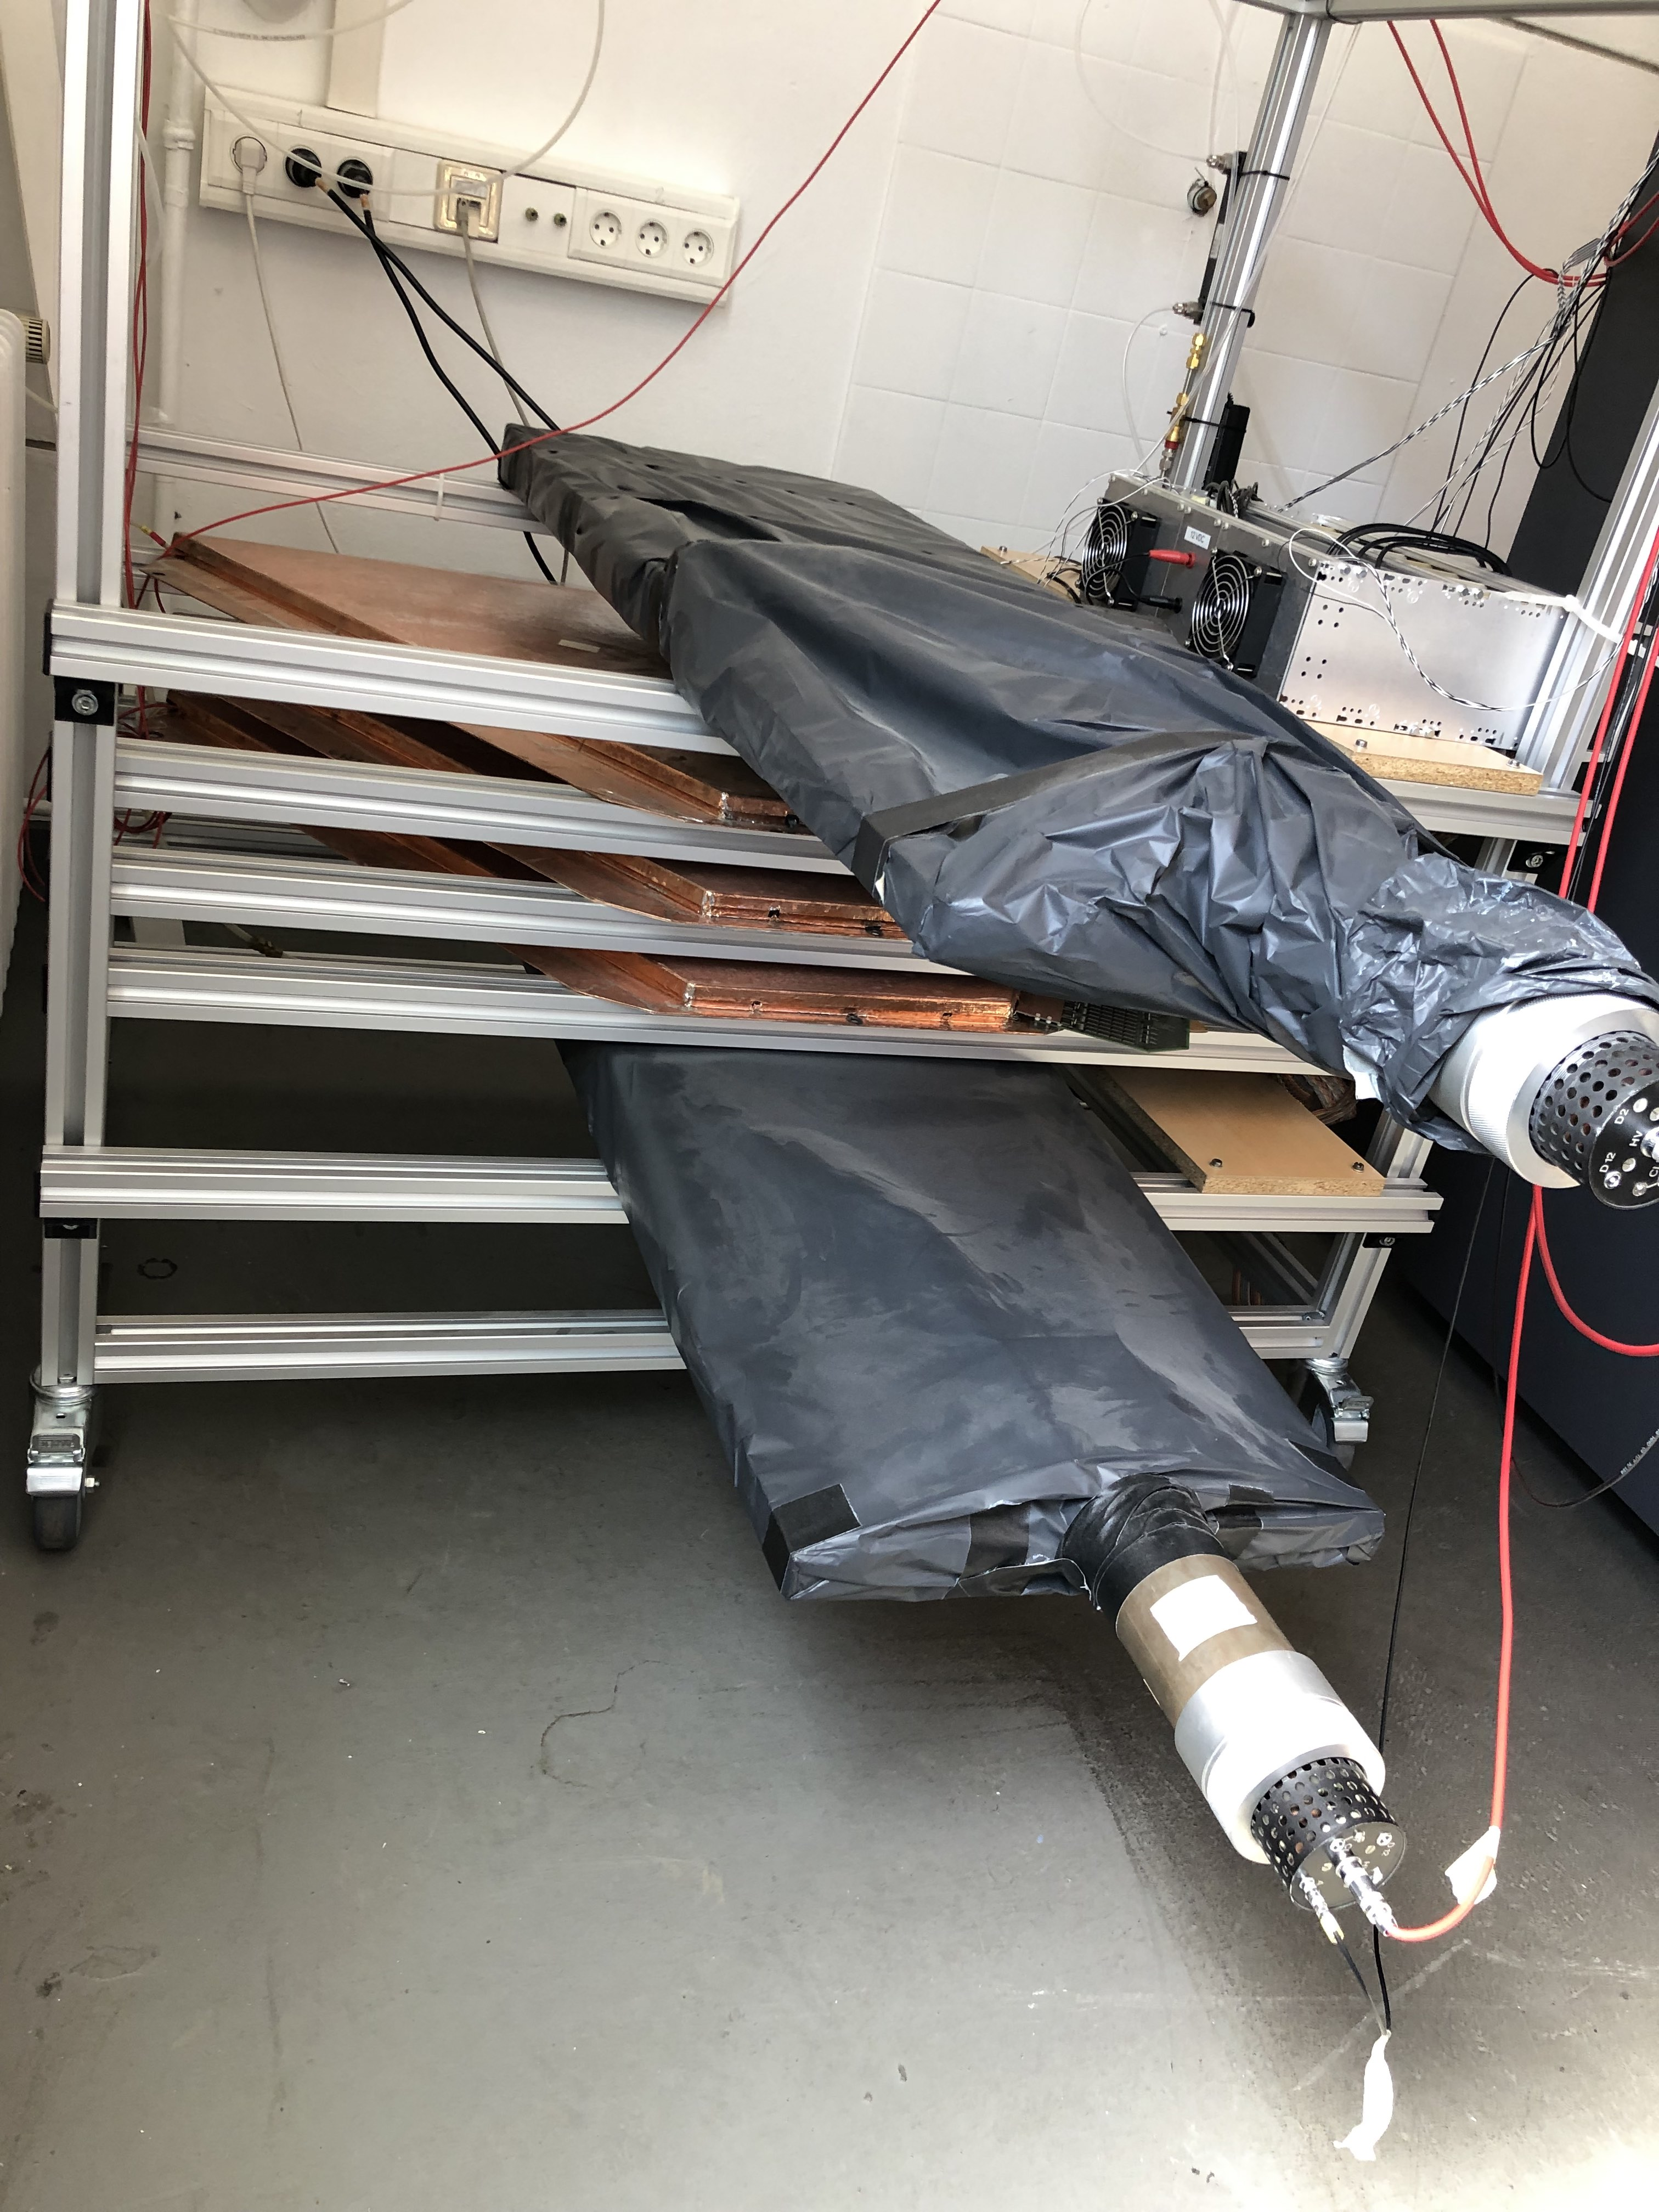
\includegraphics[width=0.5\textwidth]{setup1.jpg}
    \caption{Experimental setup with modules (copper-colored trapezoid) and PMTs (black panels).}
    \label{fig:setup1}
\end{figure}	

The modules consist of simple drift chambers. Each of these modules consists of three layers of 88 straws. The straws are a simple drift chambers, filled with a gas mixture of argon and carbon-dioxide. The radius of each straw is 3.75mm and the length ranges from 20cm to 102cm. The reason for the variable length is due to the trapezoidal shape of the module. Each of these straws is connected to readout channel in a front-end (FE) board which contains a preamplifier, a shaper and a discriminator. When the input voltage exceeds a certain threshold voltage, each of these straws give a digital output pulse. This output pulse is then time-multiplexed for six straws each, which gives an output signal with 200ns offset with respect to each other, giving a total of 1200ns readout window per event. From the FE board, the signal is fed into the TDC board to measure drift time.  

\section{Triggering system}
Since the detectors themselves do not have an internal triggering mechanism, an external one is used. This triggering system comprises of two large scintillators which are placed above and below the modules. To these scintillators, photomultiplier tubes (PMTs) are attached which registers the photon emitted by the material when a charged particles passes through and ionizes the material. This light signal is then converted to electronic pulse, which can be measured. Further, the two scintillators are operated in coincidence logic to trigger events when a muon passes both the scintillators and hence the tracking modules. 



\chapter{Procedure} \label{chap:procedure}

\section{Determination of PMT Operation Voltage}
Before making the measurements, the operation voltage for the PMT needs to be determined. In order to have a working trigger system, a high voltage needs to be set for the photomultipliers. The voltage is varied in the range of 1700-2300V. The counts measured by the lower photomultiplier are displayed on the middle counter in the electronics rack (as seen in Fig. \ref{fig:rack}). In order to reduce the statistical uncertainty, four measurements for each voltage were measured. The result is shown in Fig. \ref{fig:low_count}. A change in upper photomultiplier voltage does not affect the count. A standard error of 0.5V is taken for each reading based on the instrumentation. 

\begin{figure}[htpb]
    \centering
    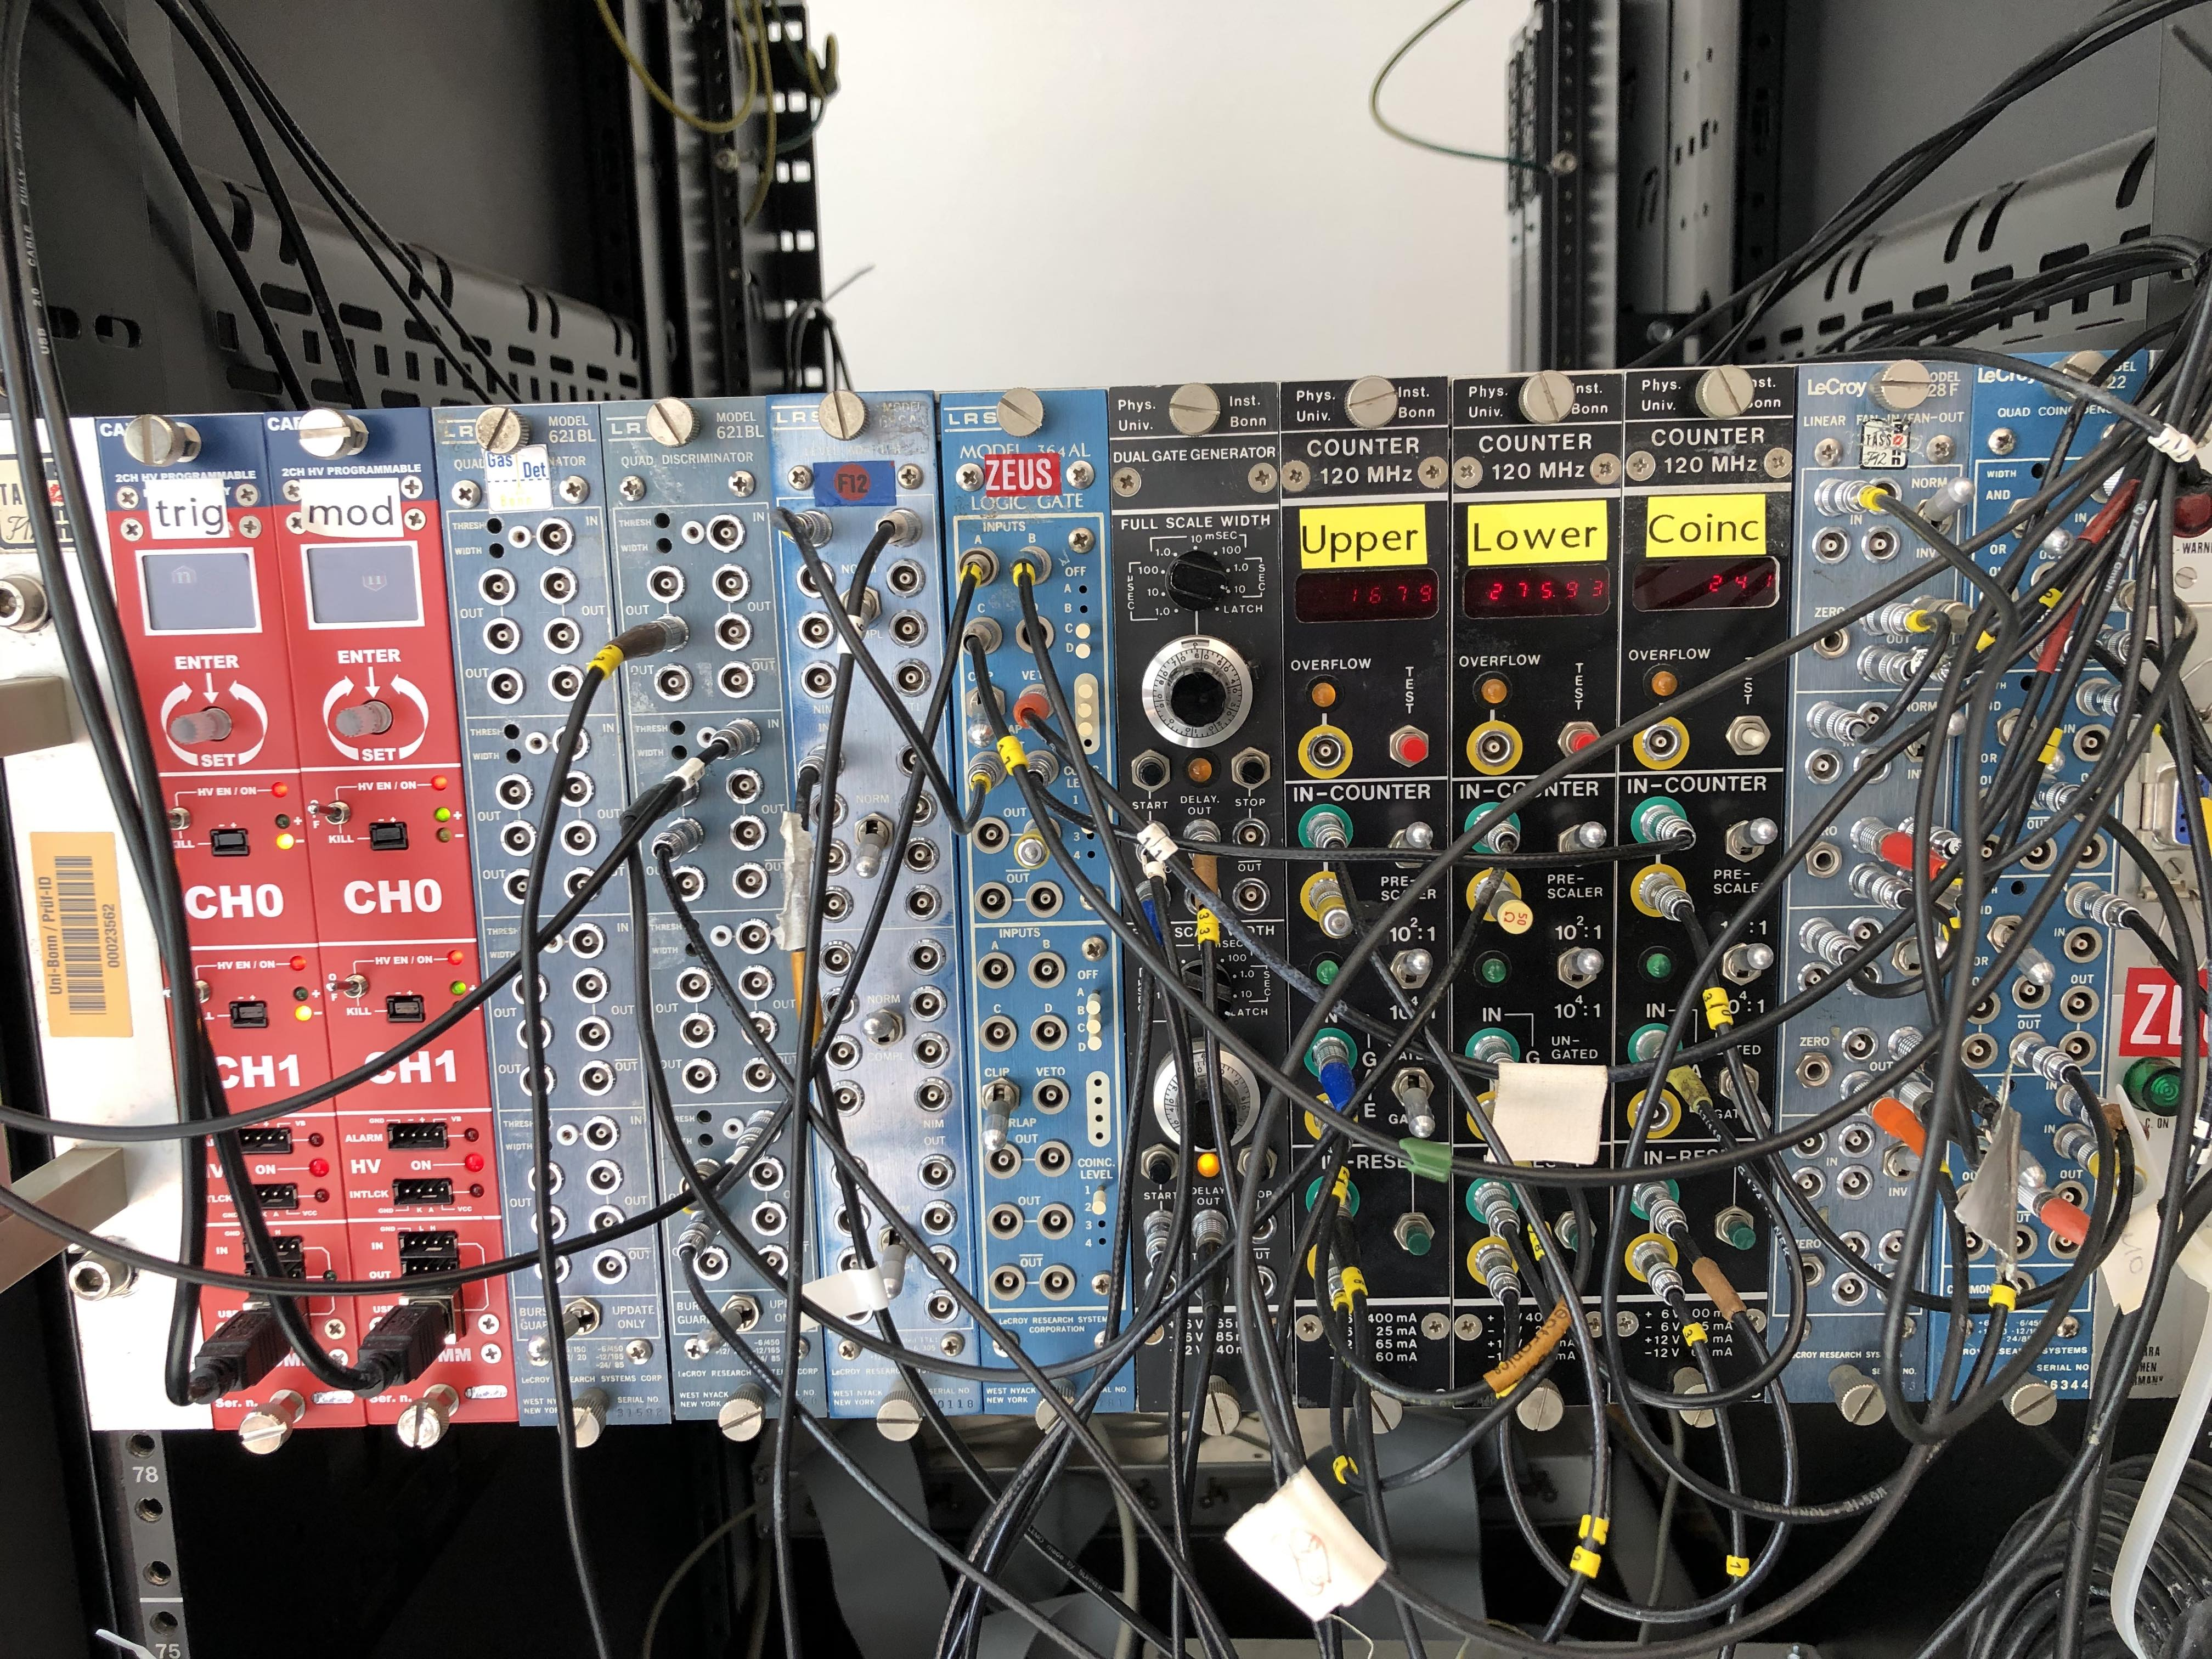
\includegraphics[width=0.5\textwidth]{rack.jpg}
    \caption{The electronic rack which displays the count for upper and lower photomultiplier and the coincidence rate.}
    \label{fig:rack}
\end{figure}	

\begin{figure}[htpb]
    \centering
    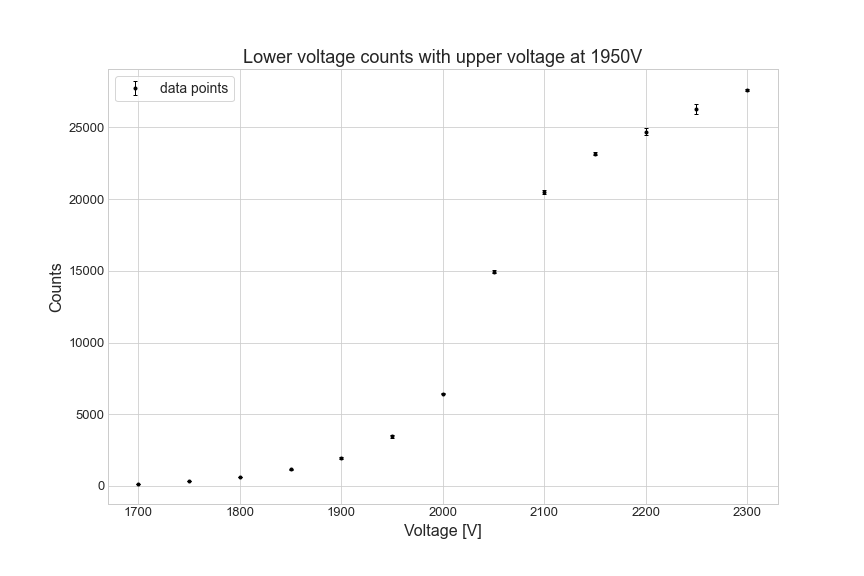
\includegraphics[width=0.8\textwidth]{low_count}
    \caption{The change in count with respect to voltage. We notice an exponential growth followed by a linear growth.}
    \label{fig:low_count}
\end{figure}	

We notice that from 1700-2050V, the behavior is exponential and after 2100V, the behavior is linear. Therefore, we choose the operating voltage for the lower photomultiplier to be 2100V, since above this value, an increase voltage leads to an increase in noise. 

Having fixed the voltage for the bottom panel, we determine the operating voltage for the upper panel. This is done by varying the voltage in the same range but this time instead of measuring the count, we measure the coincidence rate. Again, we take four measurements per voltage to reduce statistical uncertainty. The result is shown in Fig. \ref{fig:up_count}. 

\begin{figure}[htpb]
    \centering
    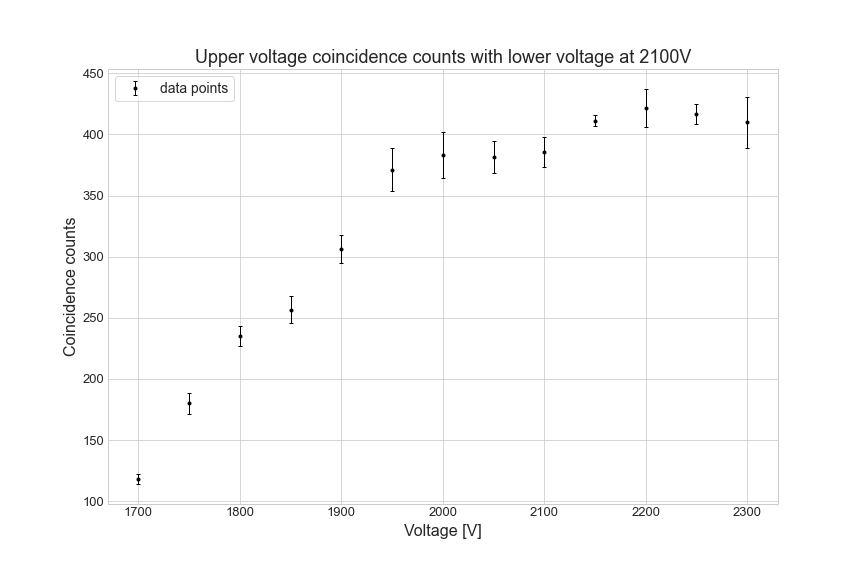
\includegraphics[width=0.8\textwidth]{up_count}
    \caption{The change in coincidence rate with respect to voltage. We notice a plateau, indicating the independence of coincidence rate.}
    \label{fig:up_count}
\end{figure}

A plateau can be seen starting after 1950V. This implies that a subsequent increase in voltage does not change the coincidence rate - the coincidence rate is independent of increase in the voltage. Therefore, we pick 2000V as the operating voltage for the upper panel. 

\section{Front-end Threshold Voltage}

Having determined the optimal operating voltage for the lower and the upper panel, the threshold voltage for front-end has to be determined. To do this, the voltage is varied 1.0-2.6V in the steps of 0.4V. An additional 2.0V reading was also taken. For each voltage, 25000 events are measured. We illustrate the typical procedure below. 

After taking the measurement for 1.0V, the following command is run:

\begin{tcolorbox}
\begin{verbatim}
StyxM2C2 -N 25000 -O TS_10V.txt --all --no-clean \ 
 -I /home/styx/data/etraxp114/te13085163152.hld
\end{verbatim}
\end{tcolorbox}

\noindent in order to process the data. The \texttt{StyxM2C2} calls the program. \texttt{-N 25000} considers only the first 25000 events to process them. \texttt{-O TS\_10V.txt} names the output file. \texttt{--all --no-clean} process the data files with \texttt{StyxM2C2} using all process steps except for the cleaning. \texttt{-I \slash home\slash styx\slash data\slash etraxp114\slash te13085163152.hld} is the input file. This is repeated for each voltage. 

To find good channels, the a monitoring root file is produced using the command: 

\begin{tcolorbox}
\begin{verbatim}
StyxMonitor TS_10V_mon.txt
\end{verbatim}
\end{tcolorbox}
\noindent This create a \texttt{TS\_10V\_mon.root} file, which can be opened via running:

\begin{tcolorbox}
\begin{verbatim}
root TS_10V_mon.root
\end{verbatim}
\end{tcolorbox}
\noindent After \texttt{root} has started, the command \texttt{new TBrowser} is used to browse through the plots and study them. To compare the results from one TDC number and one channel number, the following command is run: 

\begin{tcolorbox}
\begin{verbatim}
StyxThresholdScan 1 3 TS_10V_mon.txt TS_14V_mon.txt TS_18V_mon.txt TS_20V_mon.txt\ 
TS_22V_mon.txt TS_26V_mon.txt
\end{verbatim}
\end{tcolorbox}
\noindent This would then compare the channel 3 and TDC 1 for all the measurements. In order to analyze these plots, we run \texttt{root} again. 

The next step is to find the threshold voltage for the front-end. In order to find the optimal value, we need a compromise between low noise and high event count. The way to do this is by comparing multiple plots that we outputted in the steps mentioned above. In Fig. \ref{fig:remove_10} we see that the number of counts corresponding to 1.0V is disproportionately high. This indicates that this is due to noise. This can also be seen from the overlay plot in Fig. \ref{fig:remove_10_1}. The black line corresponds to 1.0V. A high count and non-uniform distribution is another indicator of the noise in this channel. Hence, we rule out 1.0V. 

\begin{figure}[htpb]
    \centering
    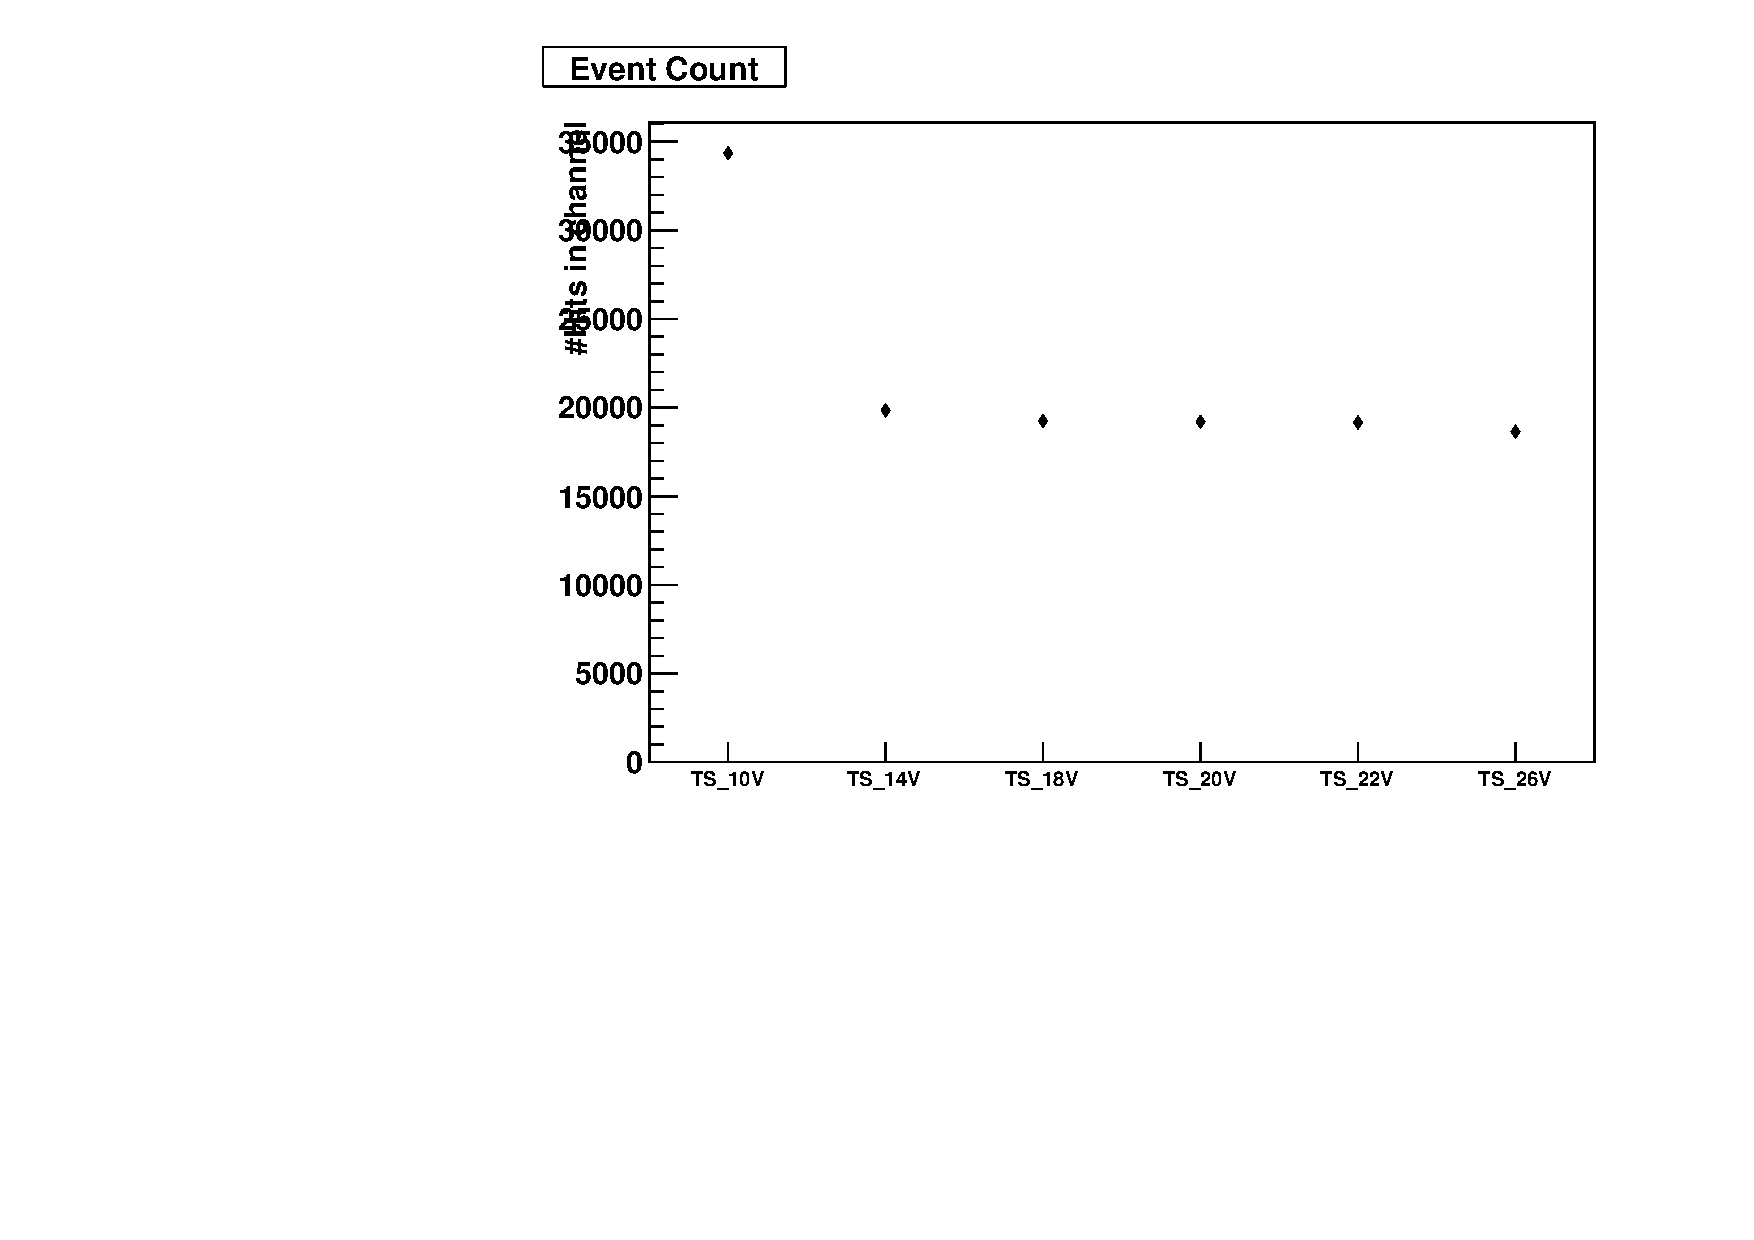
\includegraphics[width=0.65\textwidth]{StyxThresholdScan_1_11_Rate.pdf}
    \caption{Event count for different voltages for channel 11, TDC 1.}
    \label{fig:remove_10}
\end{figure}

\begin{figure}[htpb]
    \centering
    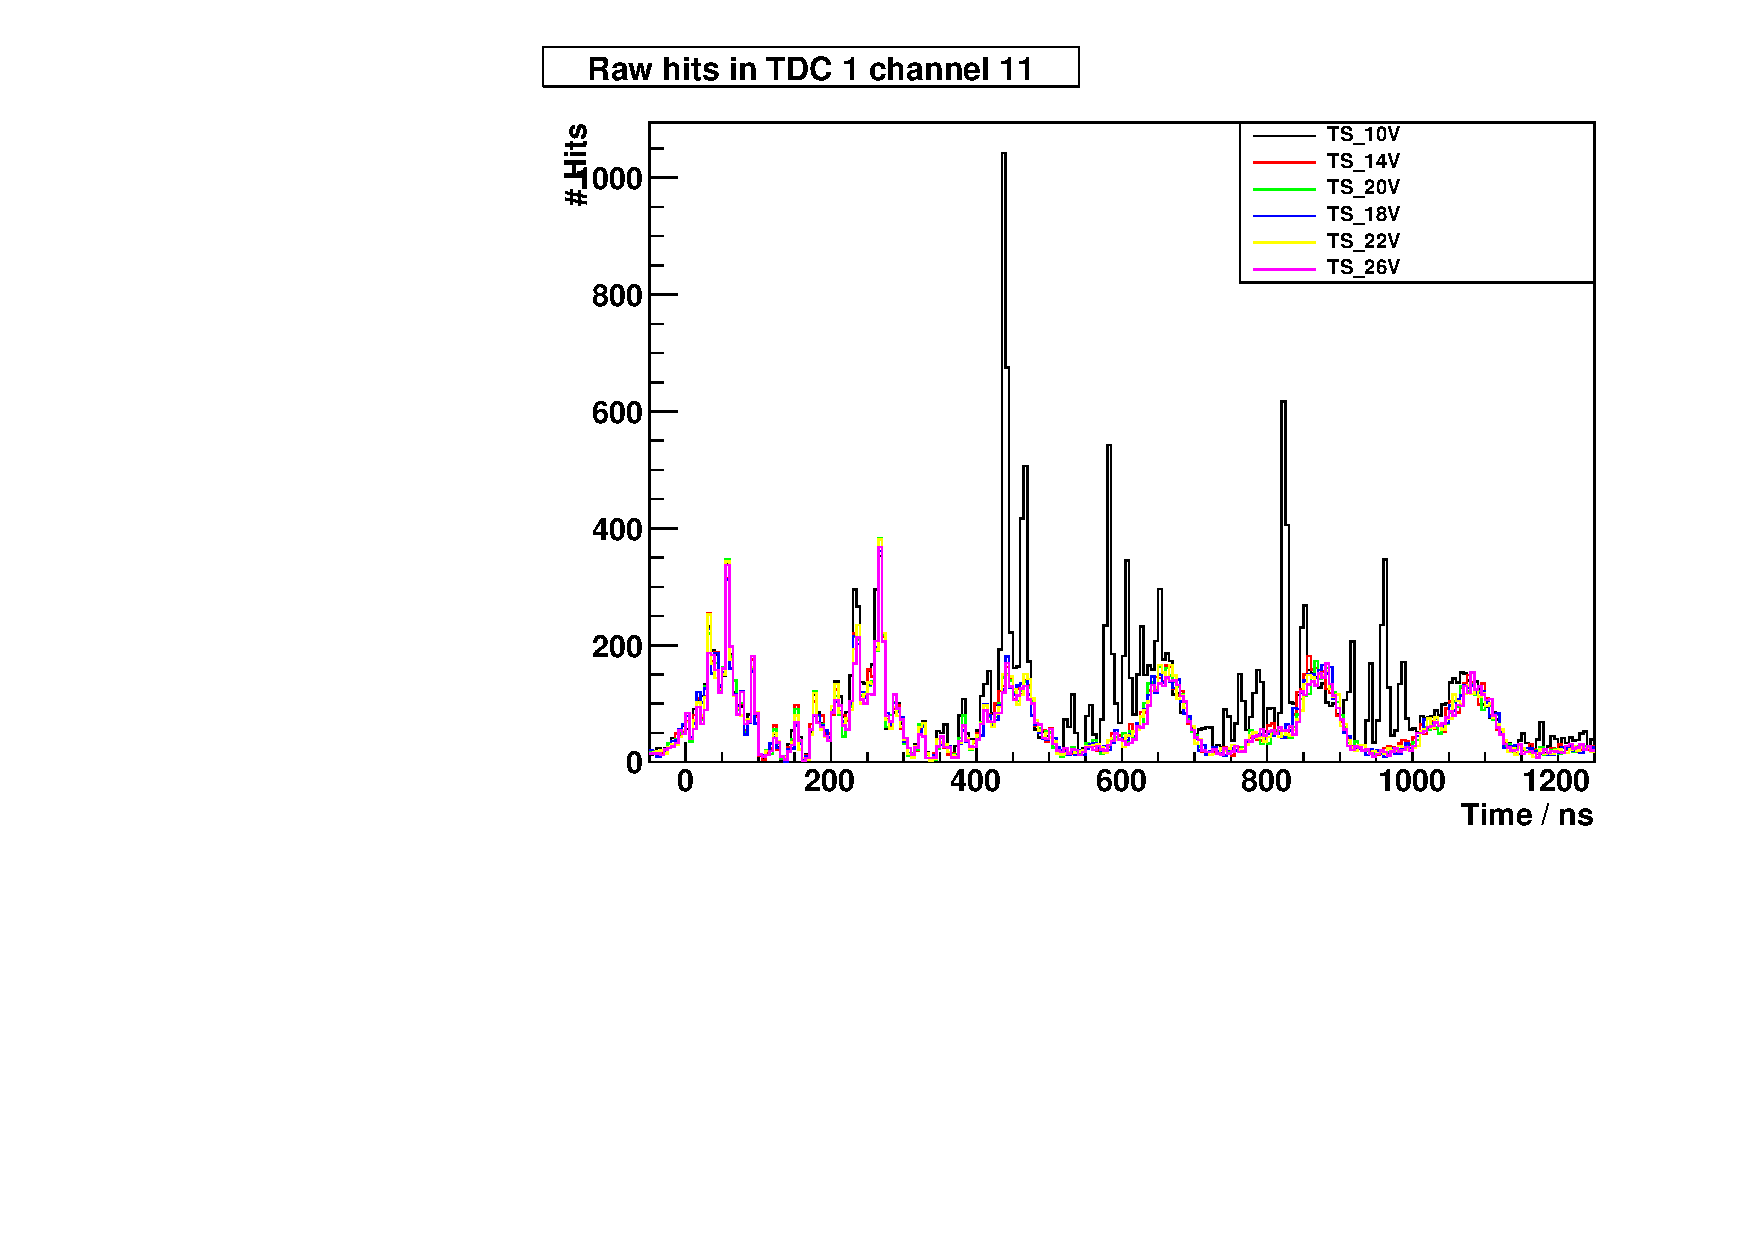
\includegraphics[width=0.65\textwidth]{StyxThresholdScan_1_11_Overlay.pdf}
    \caption{Event count for different voltages as a function of time, overlayed, for channel 11, TDC 1.}
    \label{fig:remove_10_1}
\end{figure}

Next, we look at Fig. \ref{fig:rm_below_20}. Here, we see a slight decrease in count as the voltage increases to 2.0V. After 2.0V, the value remains pretty stable. This indicates the presence of noise in voltages below 2.0V. Since the value remains constant after that, the voltages above are independent of noise, till certain extent. Hence, we rule out voltages below 2.0V and consider 2.0V as a possible candidate. 

\begin{figure}[htpb]
    \centering
    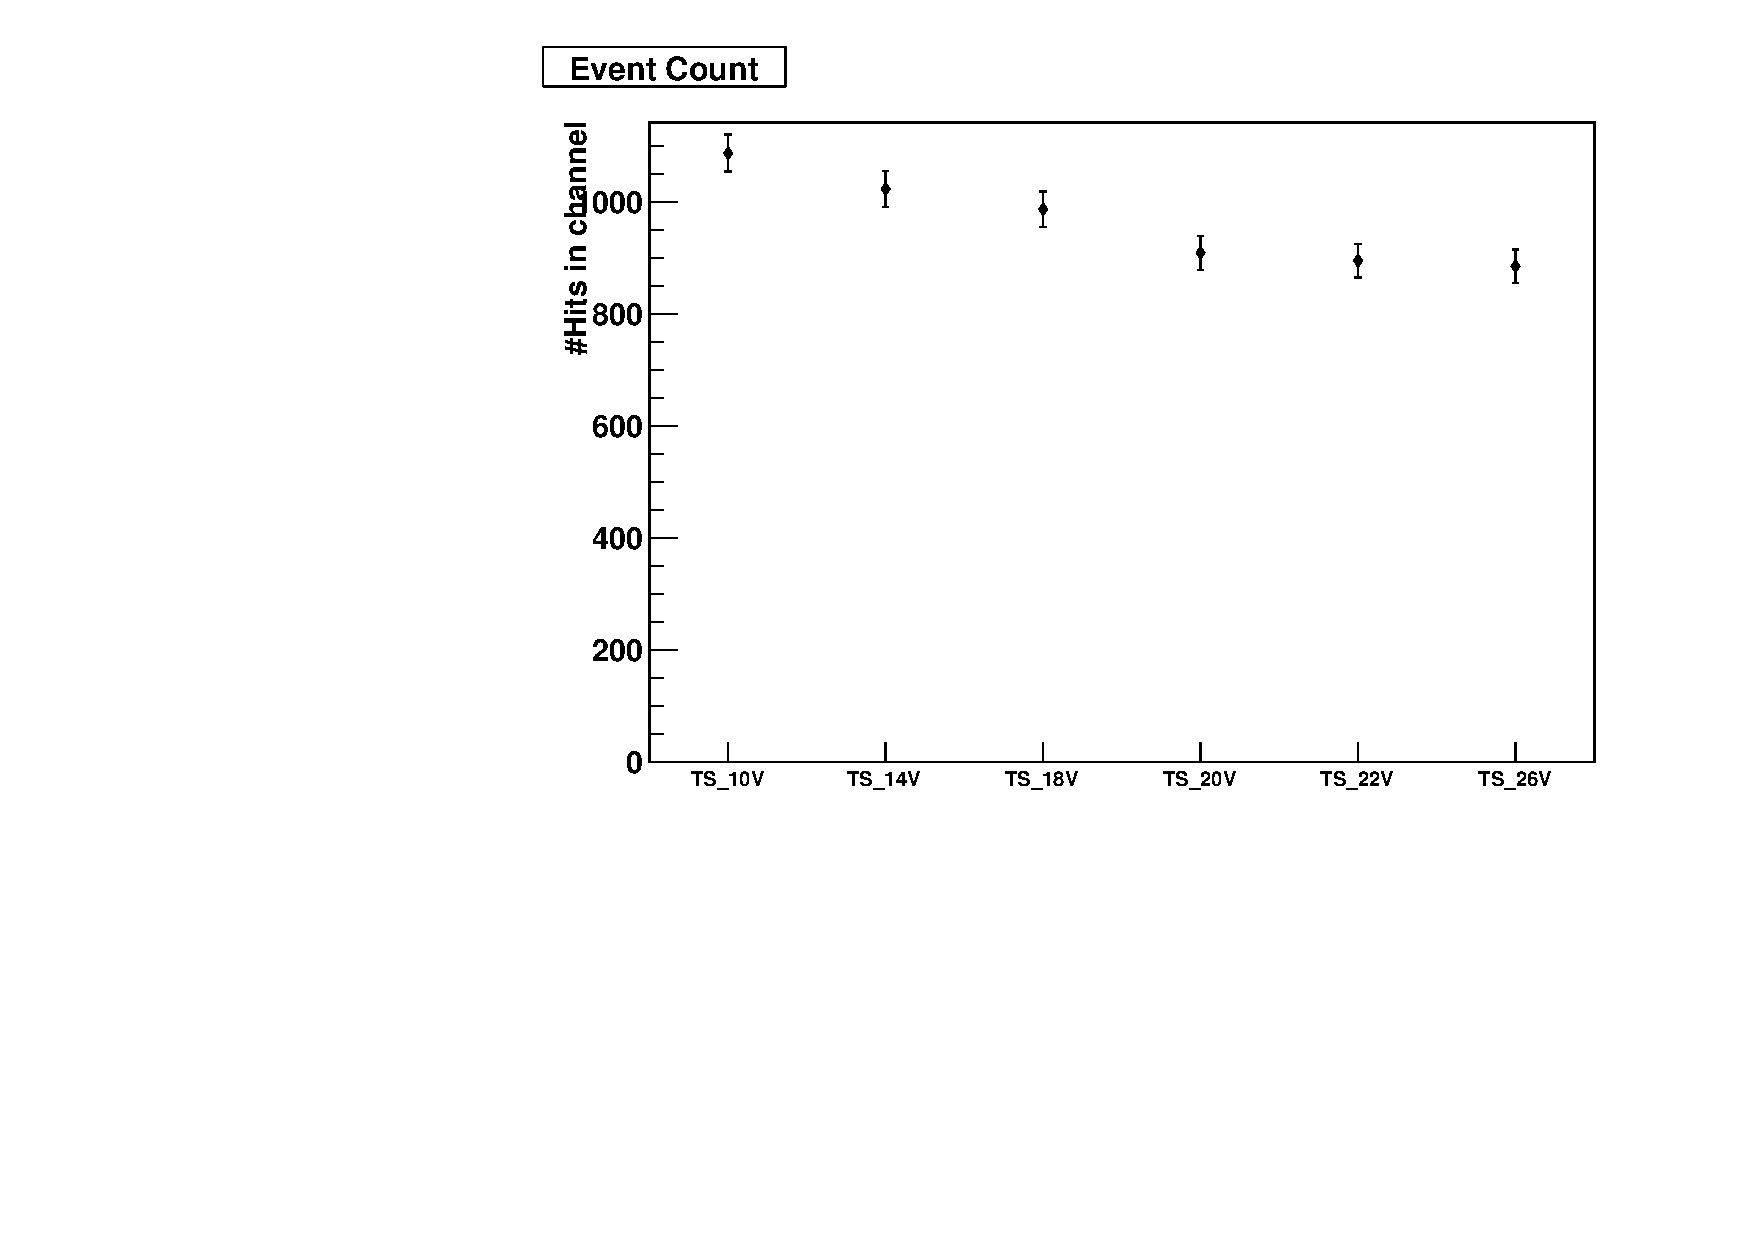
\includegraphics[width=0.65\textwidth]{StyxThresholdScan_1_3_Rate.pdf}
    \caption{Event count for different voltages for channel 3, TDC 1.}
    \label{fig:rm_below_20}
\end{figure}

Lastly, we look at Fig. \ref{fig:pick_20}. In Fig. \ref{subfig:pick_20_c}, a decrease in the count can be seen after 2.0V. Since one of our criteria was high event count, we rule out the voltages above 2.0V. Therefore, at 2.0V, we have a high event count and low noise. The corresponding overlay plot is shown in Fig. \ref{subfig:pick_20_o}. 

\begin{figure*}[htb]
	\centering
	\subfloat[Event count for different voltages. \label{subfig:pick_20_c}]{{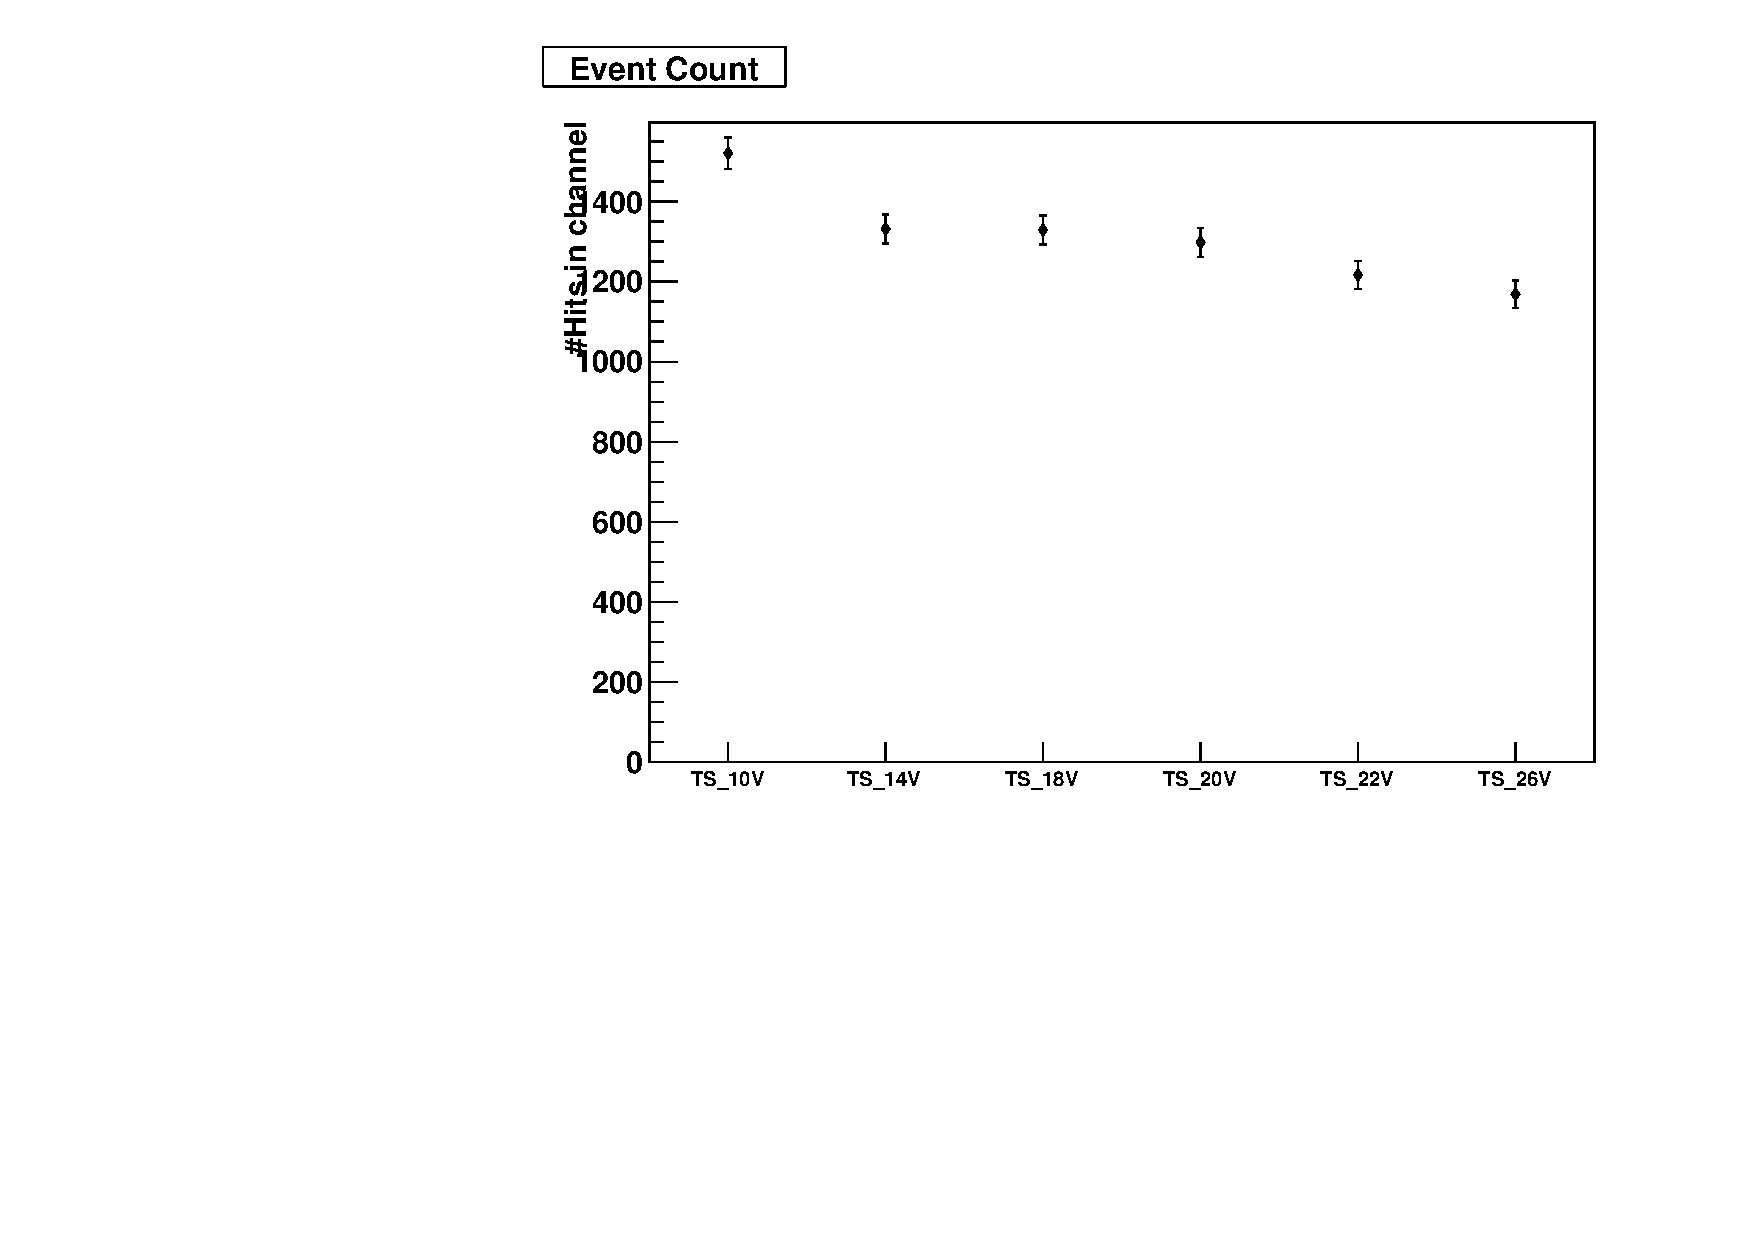
\includegraphics[width=0.47\columnwidth]{StyxThresholdScan_1_28_Rate.pdf}}}
	\quad
	\centering
	\subfloat[Event count for different voltages as a function of time, overlayed. \label{subfig:pick_20_o}]{{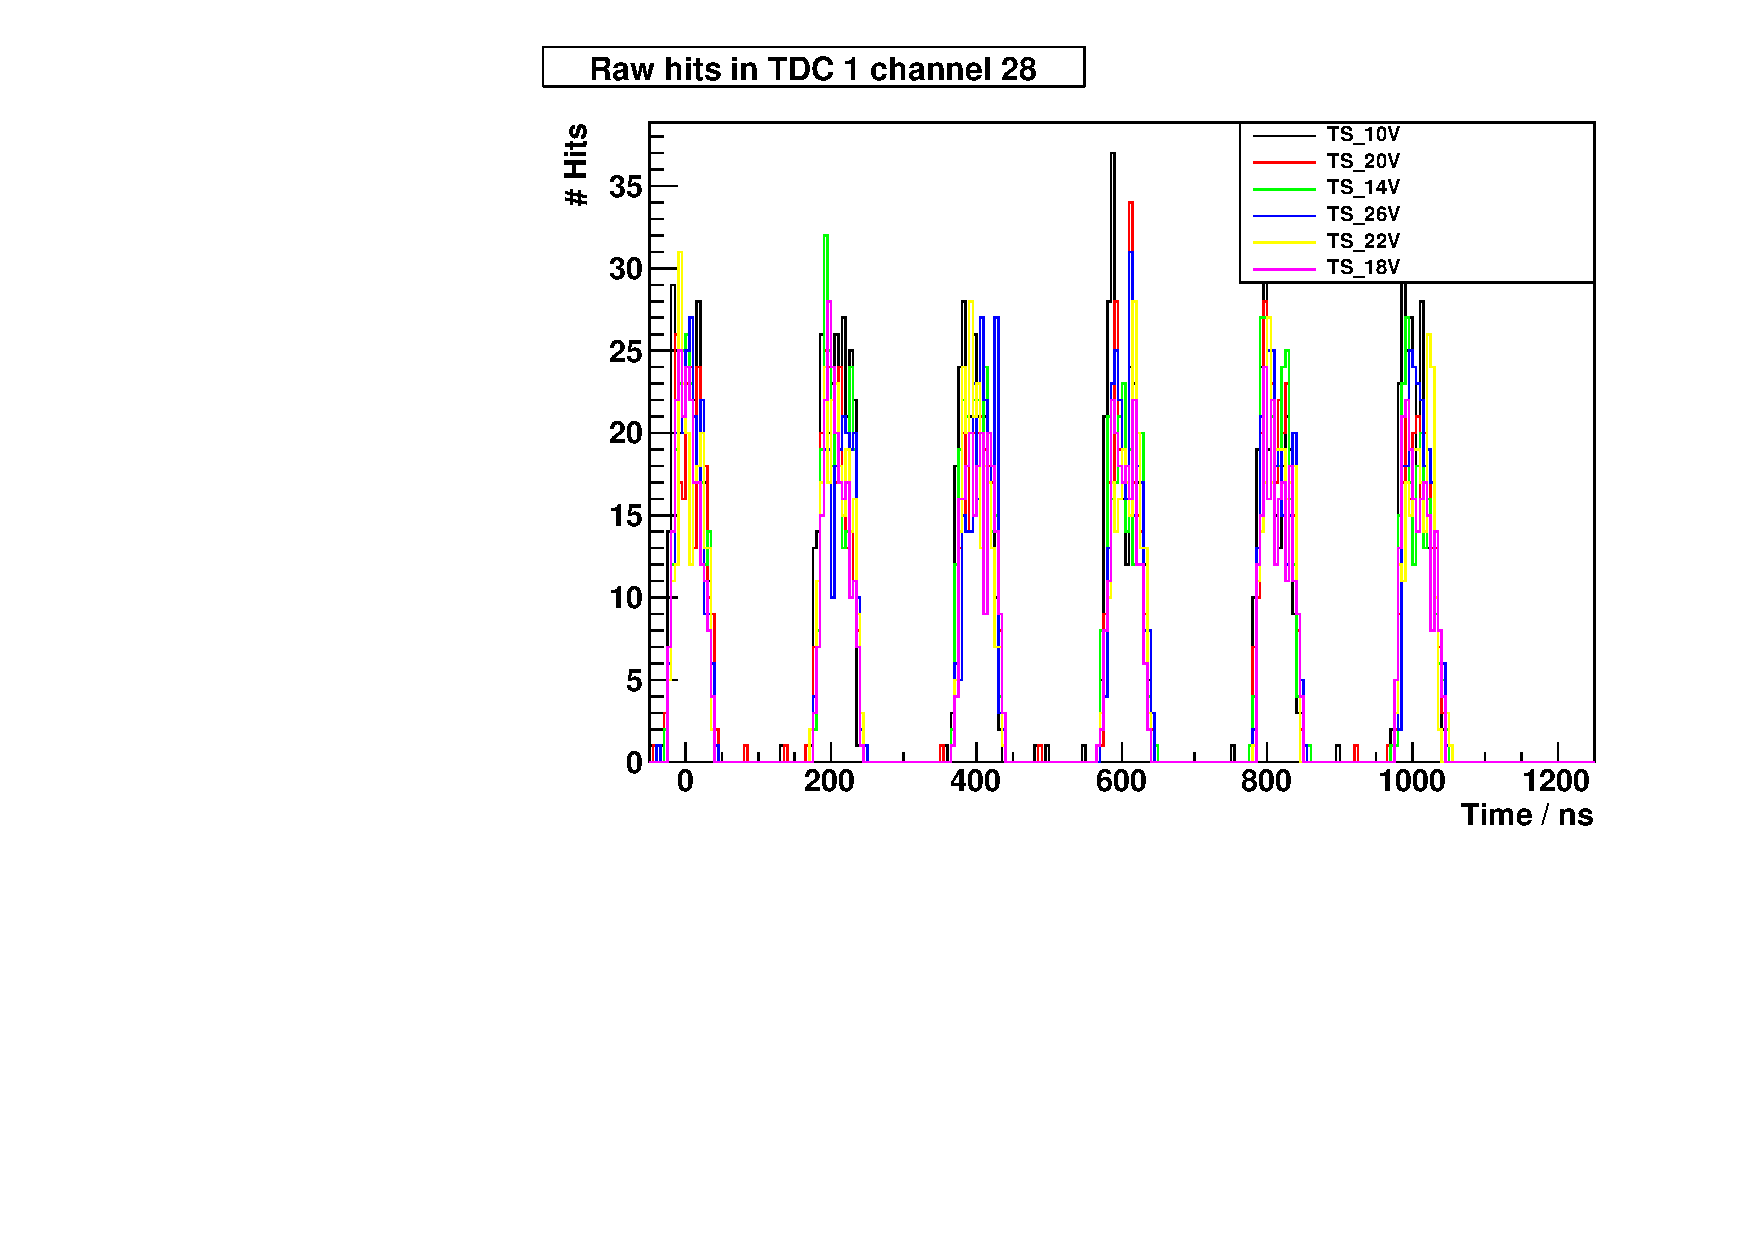
\includegraphics[width=0.47\columnwidth]{StyxThresholdScan_1_28_Overlay.pdf}}}
	\caption{Comparison plots for channel 28, TDC 1.}
	\label{fig:pick_20}
\end{figure*}


\section{Overnight Measurement}

After setting up the PMT operation voltage and the front-end threshold voltage, we then execute the program to make the measurements overnight. The data collected overnight gives high numbers of events to work with and reduces the statistical uncertainty in the analysis. The collected data was then sent to us by our tutor. 


% The experimental setup is shown in Fig. \ref{fig:setup1}. The setup consists of two major components, the modules, which are the three copper-colored trapezoids, and the trigger system, which are the two black panels. 

% \begin{figure}[htpb]
%     \centering
%     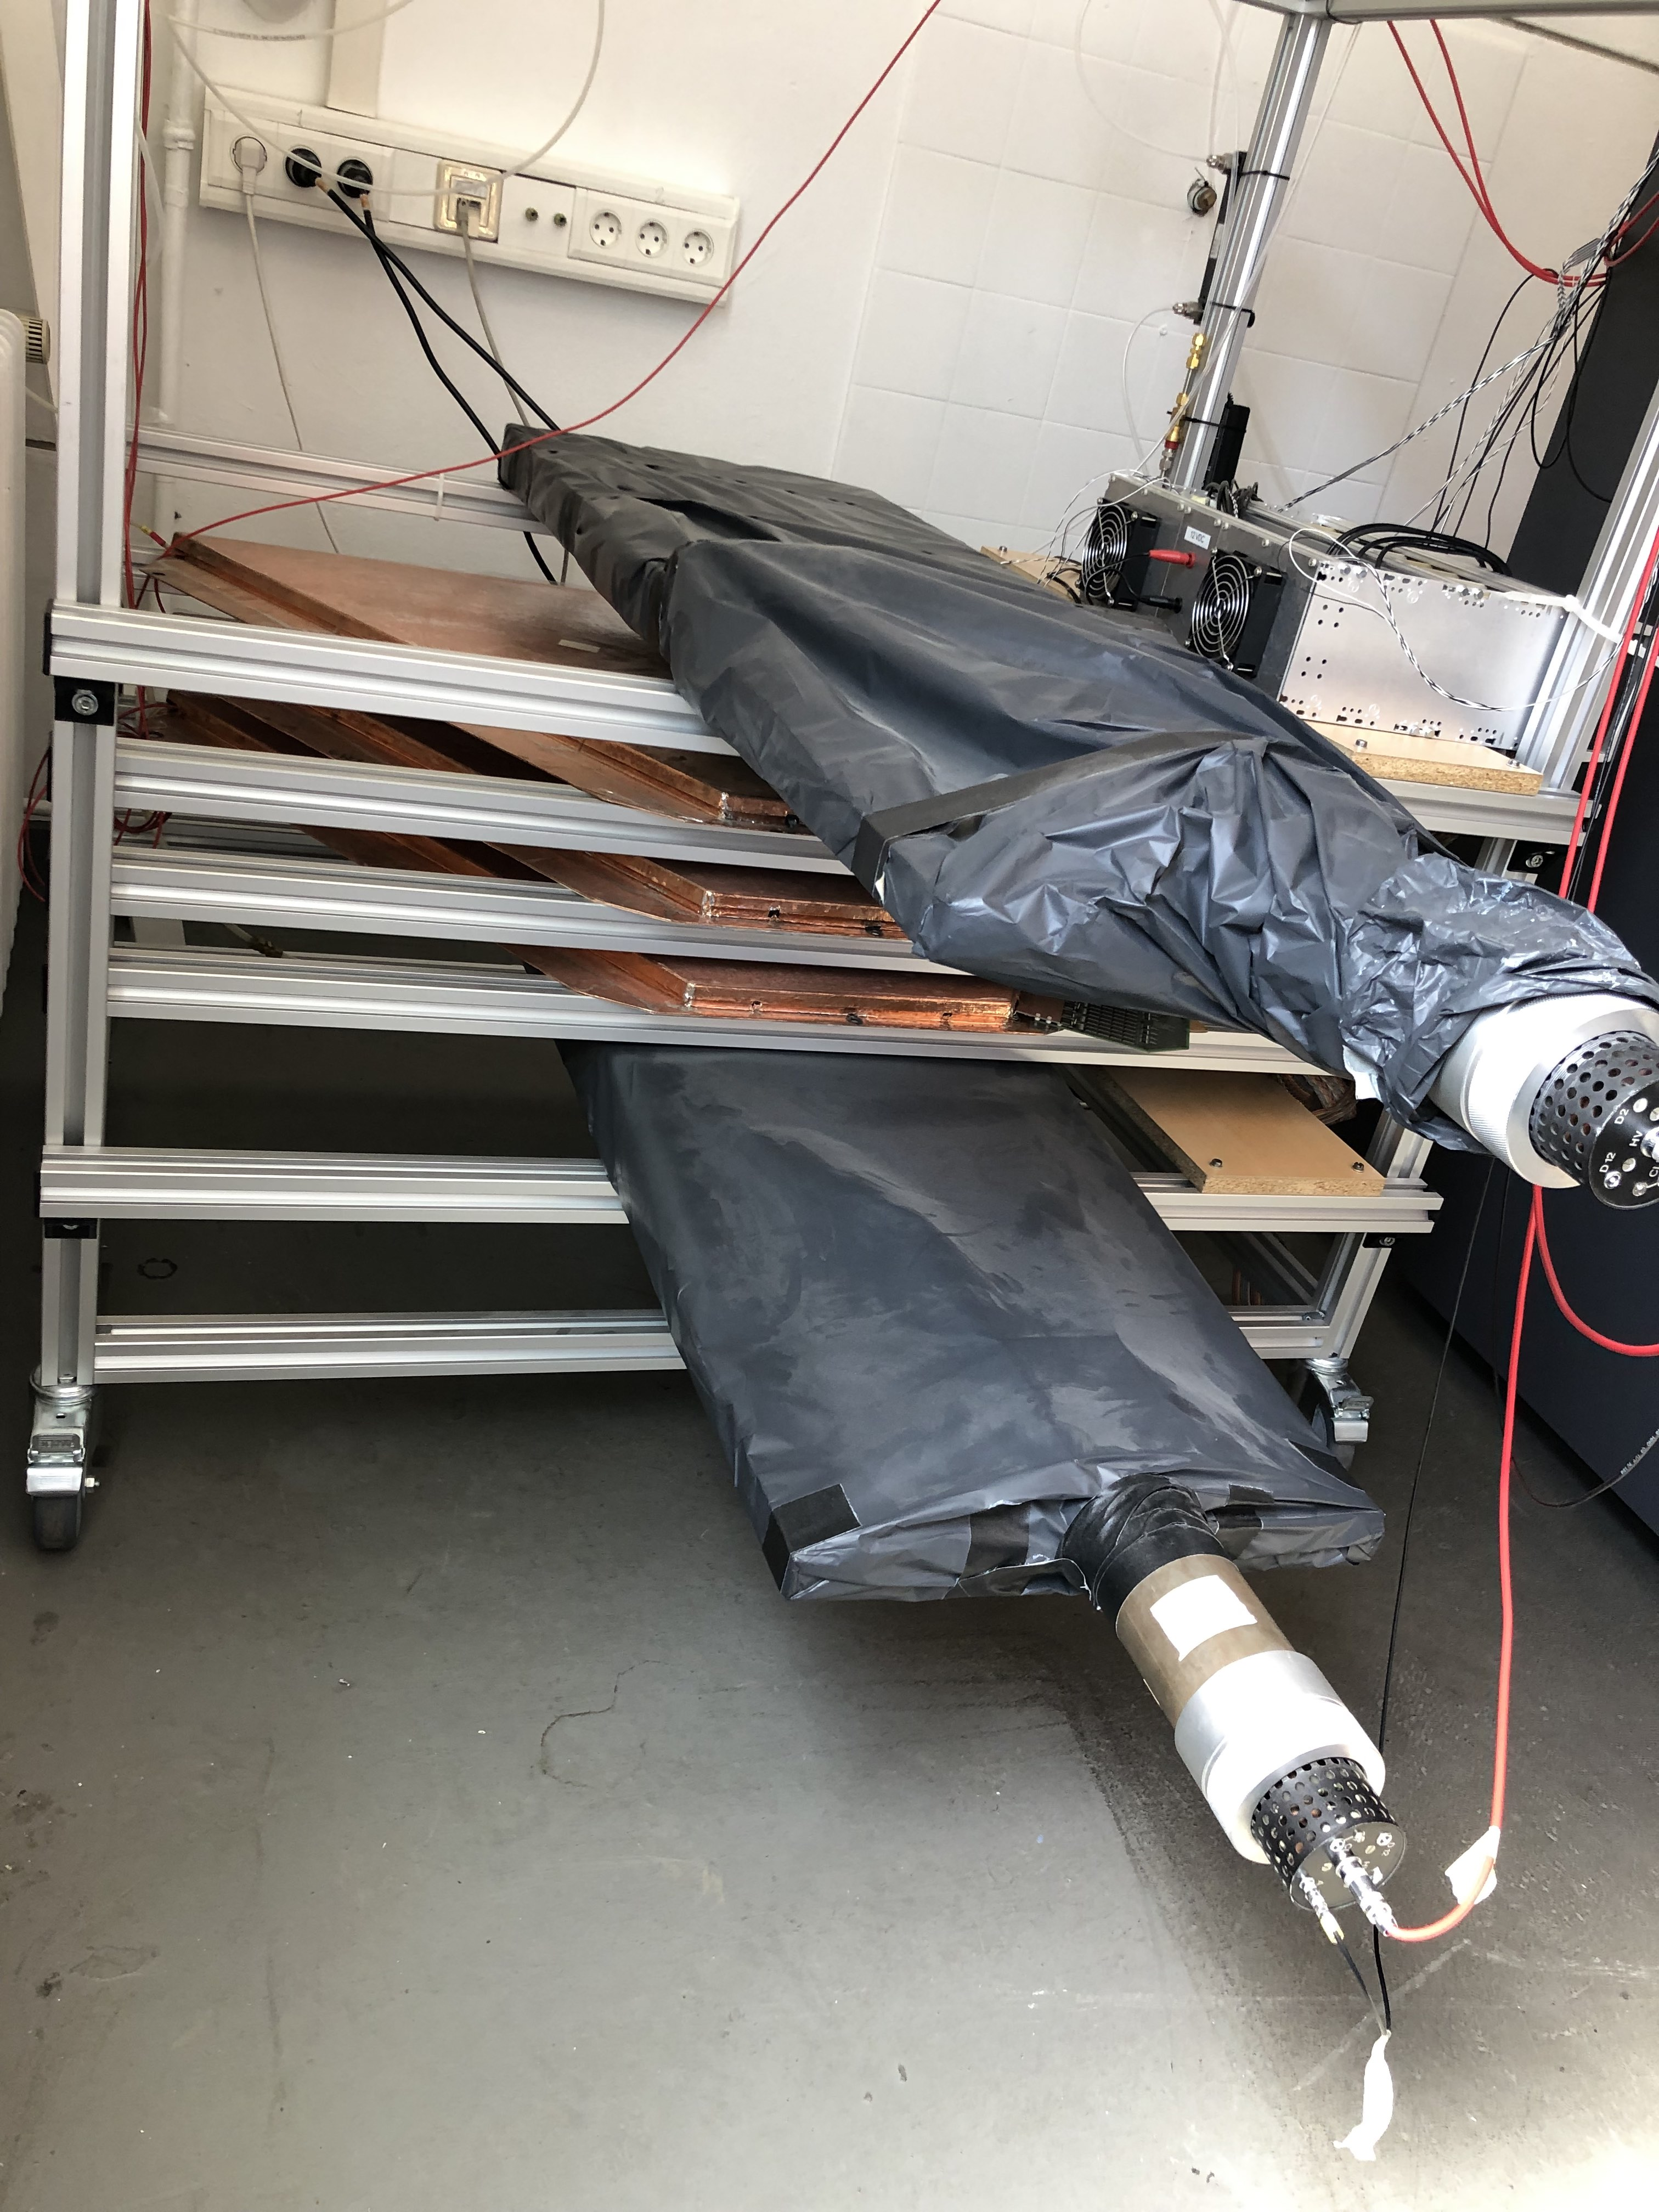
\includegraphics[width=0.6\textwidth]{setup1.jpg}
%     \caption{Experimental setup with modules (copper-colored trapezoid) and PMTs (black panels).}
%     \label{fig:setup1}
% \end{figure}	

% The modules consist of simple drift chambers. Each of these modules consists of three layers of 88 straws. The straws are a simple drift chambers, filled with a gas mixture of argon and carbon-dioxide. The radius of each straw is 3.75mm and the length ranges from 20cm to 102cm. The reason for the variable length is due to the trapezoidal shape of the module. Each of these straws is connected to readout channel in a front-end (FE) board which contains a preamplifier, a shaper and a discriminator. When the input voltage exceeds a certain threshold voltage, each of these straws give a digital output pulse. This output pulse is then time-multiplexed for six straws each, which gives an output signal with 200ns offset with respect to each other, giving a total of 1200ns readout window per event. From the FE board, the signal is fed into the TDC board to measure drift time.  

% Since the detectors themselves do not have an internal triggering mechanism, an external one is used. This triggering system comprises of two large scintillators which are placed above and below the modules. To these scintillators, photomultiplier tubes (PMTs) are attached which registers the photon emitted by the material when a charged particles passes through and ionizes the material. This light signal is then converted to electronic pulse, which can be measured. Further, the two scintillators are operated in coincidence logic to trigger events when a muon passes both the scintillators and hence the tracking modules. 

% \chapter{Procedure}

% \section{Determination of PMT Operation Voltage}
% Before making the measurements, the operation voltage for the PMT needs to be determined. In order to have a working trigger system, a high voltage needs to be set for the photomultipliers. The voltage is varied in the range of 1700-2300V. The counts measured by the lower photomultiplier are displayed on the middle counter in the electronics rack (as seen in Fig. \ref{fig:rack}). In order to reduce the statistical uncertainty, four measurements for each voltage were measured. The result is shown in Fig. \ref{fig:low_count}. A change in upper photomultiplier voltage does not affect the count. A standard error of 0.5V is taken for each reading based on the instrumentation. 

% \begin{figure}[htpb]
%     \centering
%     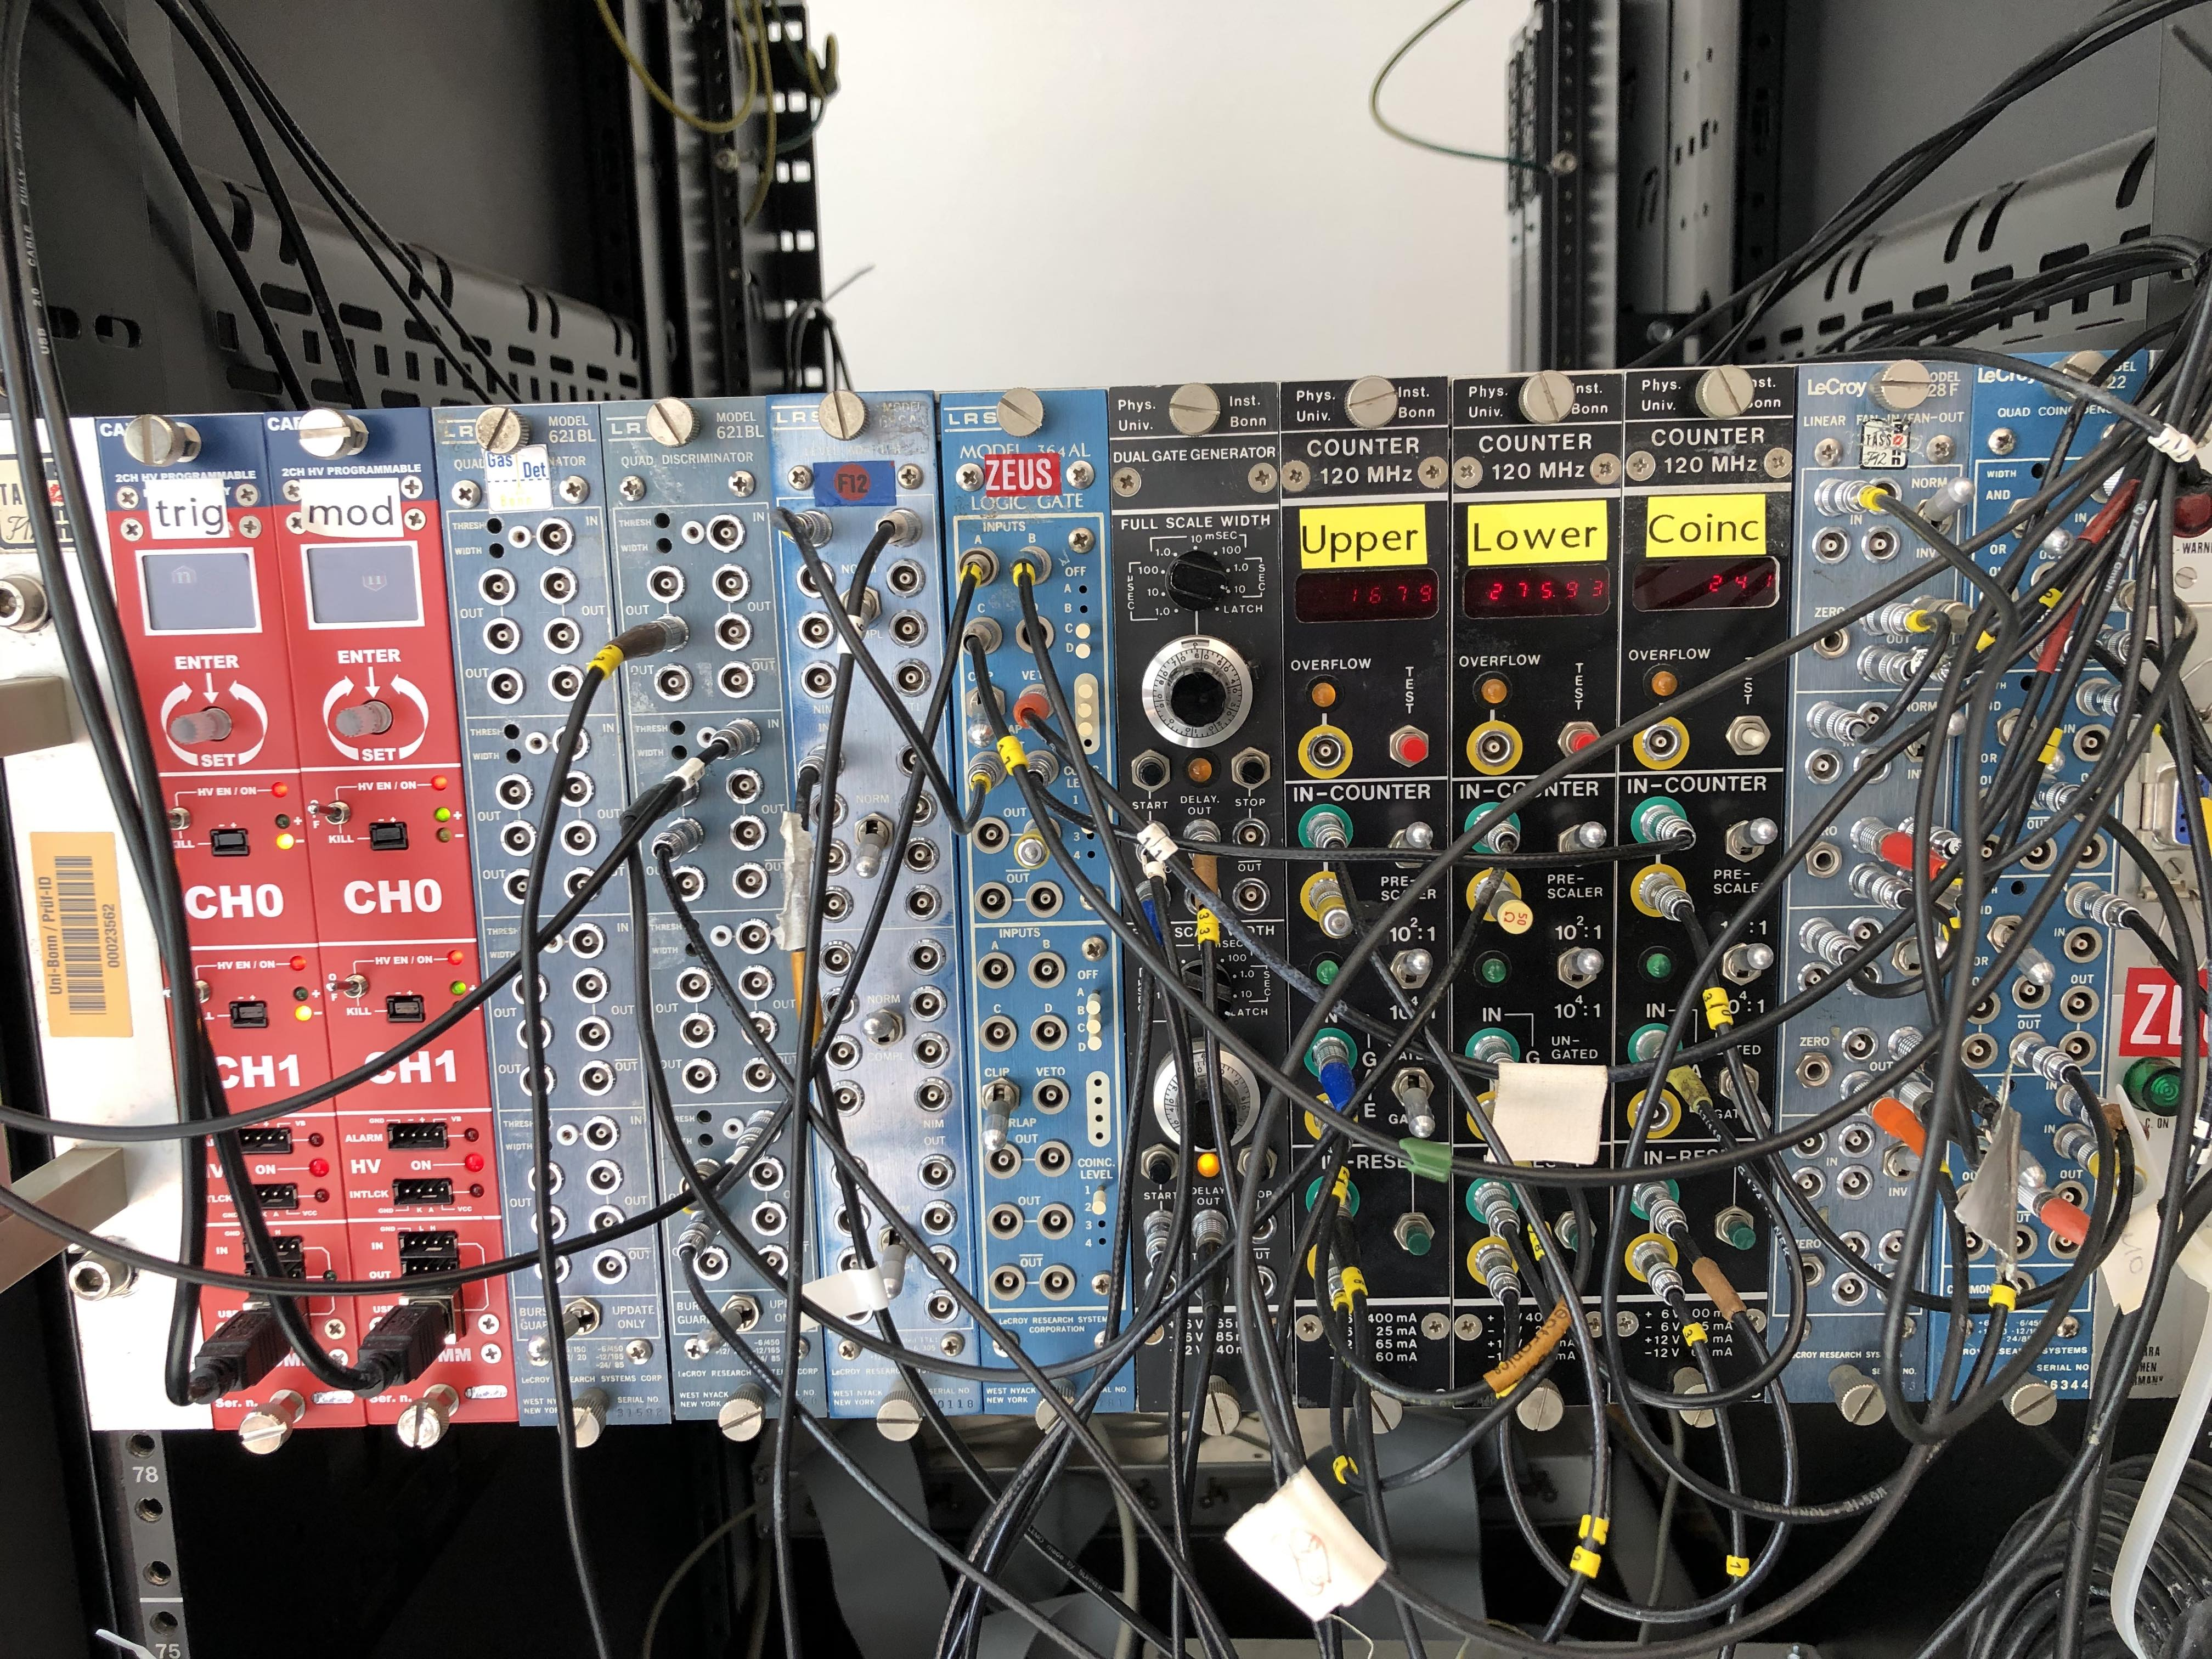
\includegraphics[width=0.6\textwidth]{rack.jpg}
%     \caption{The electronic rack which displays the count for upper and lower photomultiplier and the coincidence rate.}
%     \label{fig:rack}
% \end{figure}	

% \begin{figure}[htpb]
%     \centering
%     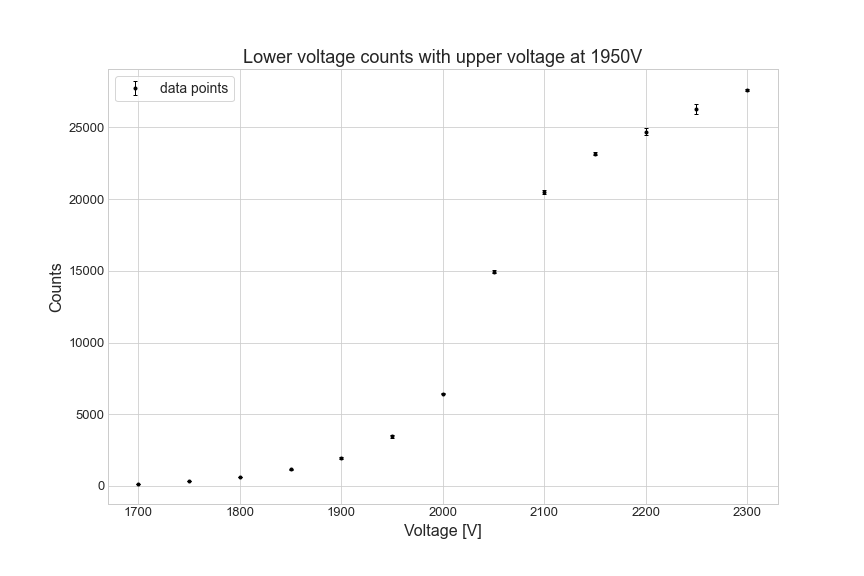
\includegraphics[width=0.8\textwidth]{low_count}
%     \caption{The change in count with respect to voltage. We notice an exponential growth followed by a linear growth.}
%     \label{fig:low_count}
% \end{figure}	

% We notice that from 1700-2050V, the behavior is exponential and after 2100V, the behavior is linear. Therefore, we choose the operating voltage for the lower photomultiplier to be 2100V, since above this value, an increase voltage leads to an increase in noise. 

% Having fixed the voltage for the bottom panel, we determine the operating voltage for the upper panel. This is done by varying the voltage in the same range but this time instead of measuring the count, we measure the coincidence rate. Again, we take four measurements per voltage to reduce statistical uncertainty. The result is shown in Fig. \ref{fig:up_count}. 

% \begin{figure}[htpb]
%     \centering
%     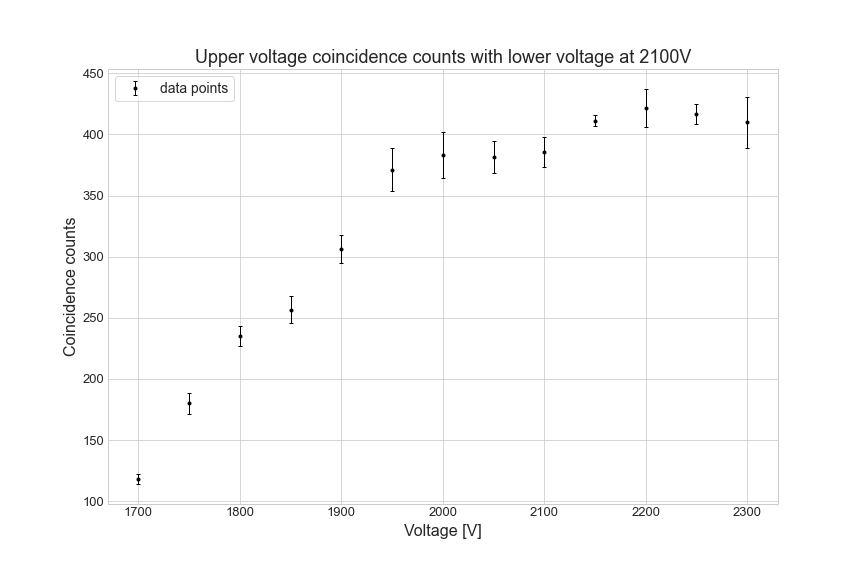
\includegraphics[width=0.8\textwidth]{up_count}
%     \caption{The change in coincidence rate with respect to voltage. We notice a plateau, indicating the independence of coincidence rate.}
%     \label{fig:up_count}
% \end{figure}

% A plateau can be seen starting after 1950V. This implies that a subsequent increase in voltage does not change the coincidence rate - the coincidence rate is independent of increase in the voltage. Therefore, we pick 2000V as the operating voltage for the upper panel. 

% \section{Front-end Threshold Voltage}

% Having determined the optimal operating voltage for the lower and the upper panel, the threshold voltage for front-end has to be determined. To do this, the voltage is varied 1.0-2.6V in the steps of 0.4V. An additional 2.0V reading was also taken. For each voltage, 25000 events are measured. We illustrate the typical procedure below. 

% After taking the measurement for 1.0V, the following command is run:

% \begin{tcolorbox}
% \begin{verbatim}
% StyxM2C2 -N 25000 -O TS_10V.txt --all --no-clean \ 
%  -I /home/styx/data/etraxp114/te13085163152.hld
% \end{verbatim}
% \end{tcolorbox}

% in order to process the data. The \texttt{StyxM2C2} calls the program. \texttt{-N 25000} considers only the first 25000 events to process them. \texttt{-O TS\_10V.txt} names the output file. \texttt{--all --no-clean} process the data files with \texttt{StyxM2C2} using all process steps except for the cleaning. \texttt{-I \slash home\slash styx\slash data\slash etraxp114\slash te13085163152.hld} is the input file. This is repeated for each voltage. 

% To find good channels, the a monitoring root file is produced using the command: 

% \begin{tcolorbox}
% \begin{verbatim}
% StyxMonitor TS_10V_mon.txt
% \end{verbatim}
% \end{tcolorbox}
% This create a \texttt{TS\_10V\_mon.root} file, which can be opened via running:

% \begin{tcolorbox}
% \begin{verbatim}
% root TS_10V_mon.root
% \end{verbatim}
% \end{tcolorbox}
% After \texttt{root} has started, the command \texttt{new TBrowser} is used to browse through the plots and study them. To compare the results from one TDC number and one channel number, the following command is run: 

% \begin{tcolorbox}
% \begin{verbatim}
% StyxThresholdScan 1 3 TS_10V_mon.txt TS_14V_mon.txt TS_18V_mon.txt TS_20V_mon.txt\ 
% TS_22V_mon.txt TS_26V_mon.txt
% \end{verbatim}
% \end{tcolorbox}
% This would then compare the channel 3 and TDC 1 for all the measurements. 


% \section{Overnight Measurement}



\chapter{Calibration} \label{chap:calib}

In this chapter, we describe the calibration process, namely the straw-by-straw calibration method, performed 
on the raw data measured overnight. Such calibration was applied to our data as the measured drift times 
are individually offset for each straw and as such a correction to this offset was required.

\section{Procedure} \label{sec:calib_proc}

The straw-by-straw calibration method finds the starting point of the drift time distribution and shifts it to 
zero time in order to correct for the offset of the drift times. This is performed by fitting the rising edge of the 
distribution to determine the starting point of the distribution. See Fig. \ref{fig:calib_drift_fit} for an example of the fitting process of the 
drift time distribution. The calibration also marks straws as hot, dead, or continuous if the distribution of that straw 
does not have the expected shape. \par 

\begin{figure*}[!h]
	\centering
	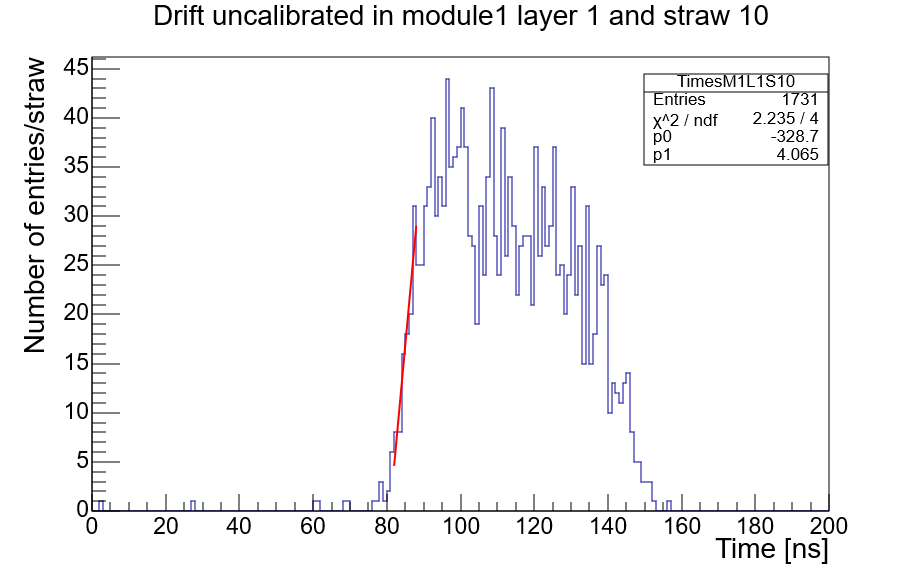
\includegraphics[width=0.6\textwidth]{calib_drift_m1l1s10_fit.png}
	\caption{Example of the fitting process. A linear fit is applied on the rising edge of the distribution for the calibration process. The uncalibrated drift time distribution
	 for Module 1, Layer 1 and Straw 10 is shown. }
	\label{fig:calib_drift_fit}
\end{figure*}

In order to run the calibration, we use the first 300 000 events through \texttt{StyxM2C2} as mentioned in 
Sec. \ref{sec:fe_threshhold} using the following command:
\begin{tcolorbox}
	\texttt{StyxM2C2 -N 300000 -O CalibM2C2300k.txt -I ../te22132161802.hld --no-clean --all}
\end{tcolorbox}
where \texttt{te22132161802.hld} contains the raw data from the overnight measurement. The calibration was then performed using the \texttt{StyxCalibration} 
tool provided by running the following command:
\begin{tcolorbox}
	\texttt{StyxM2C2 -A CalibStrawByStraw -O CalibStraw300k -I CalibM2C2300k.txt}
\end{tcolorbox}
where the \texttt{CalibStrawByStraw} algorithm was selected. 

\section{Results} \label{sec:calib_results}

We then observed the plots generated by the ROOT output file and compared the difference between the uncalibrated and 
calibrated data. Fig. \ref{fig:calib_drift_layer} show the uncalibrated and calibrated drift time distributions obtained for Module 1, Layer 1 and 
Module 3, Layer 1. The last configuration was chosen as the distribution from the uncalibrated data showed the most background, and the first 
configuration was chosen for comparison with the other distribution. \par

\begin{figure*}[htb!]
	\centering
	\subfloat[Module 1, Layer 1 (Uncalibrated) \label{subfig:drift_layer_m1l1uc}]{{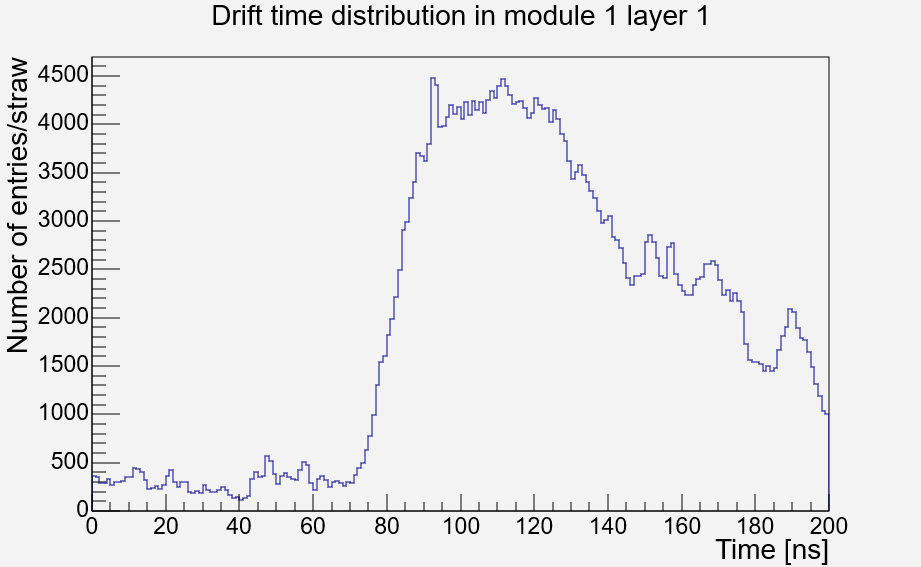
\includegraphics[width=0.47\columnwidth]{uncalib_drift_m1l1.png}}}
	\quad
	\centering
	\subfloat[Module 1, Layer 1 (Calibrated) \label{subfig:drift_layer_m1l1c}]{{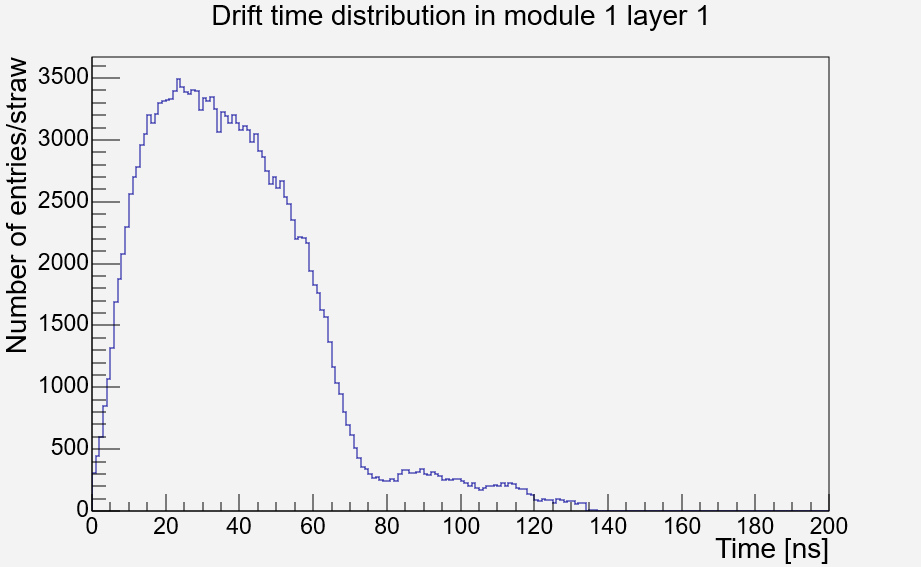
\includegraphics[width=0.47\columnwidth]{calib_drift_m1l1.png}}}
	\quad
	\centering
	\subfloat[Module 3, Layer 1 (Uncalibrated) \label{subfig:drift_layer_m3l1uc}]{{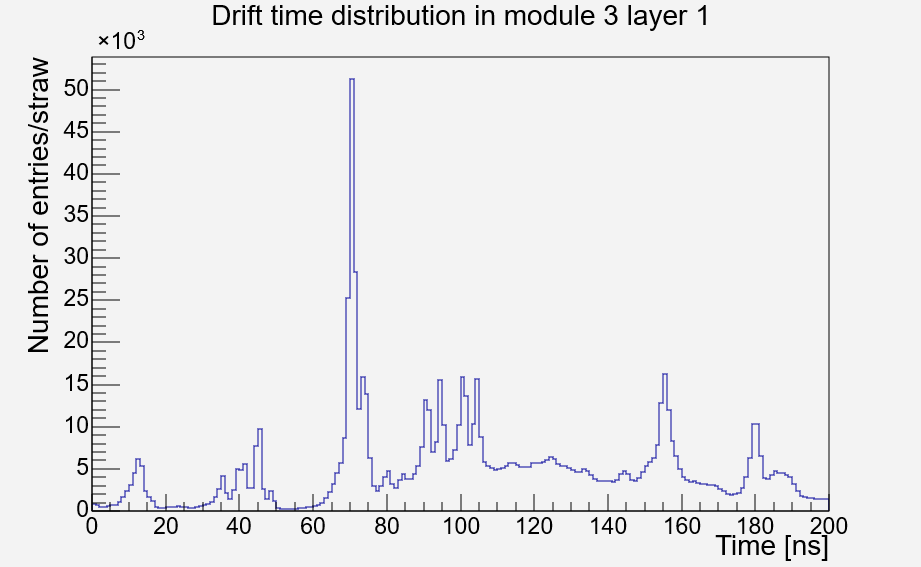
\includegraphics[width=0.47\columnwidth]{uncalib_drift_m3l1.png}}}
	\quad
	\centering
	\subfloat[Module 3, Layer 1 (Calibrated) \label{subfig:drift_layer_m3l1c}]{{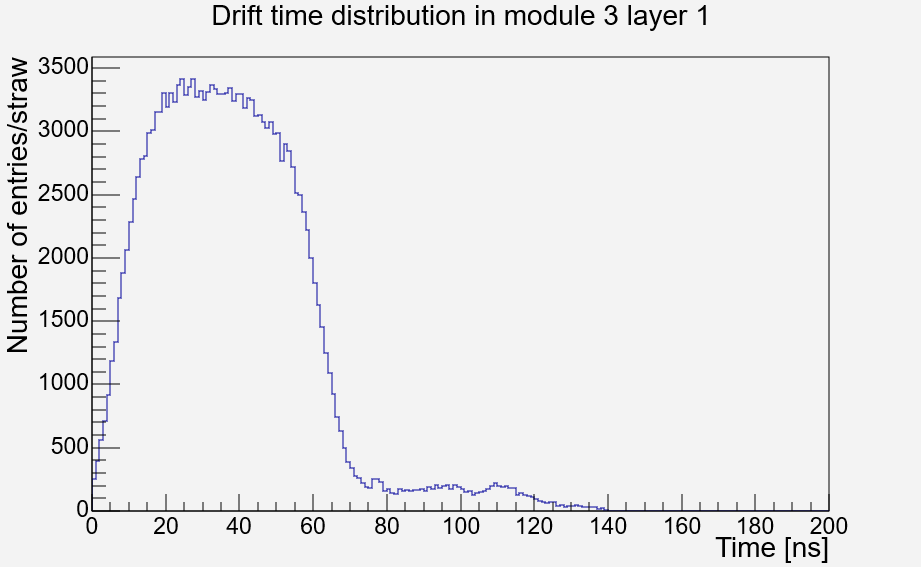
\includegraphics[width=0.47\columnwidth]{calib_drift_m3l1.png}}}
	\caption{The uncalibrated (left) and calibrated (right) drift time 
	distributions for Module 1, Layer 1 (top) and Module 3, Layer 1 (bottom).}
	\label{fig:calib_drift_layer}
\end{figure*}

By comparing between the uncalibrated and calibrated distribution for Module 1, Layer 1 (Fig. \ref{subfig:drift_layer_m1l1uc} and \ref{subfig:drift_layer_m1l1c})
, we see that the starting point of the distribution observed at approximately $\SI{70}{\nano\second}$ has been shifted to $\sim \SI{0}{\nano\second}$, 
indicating that the calibration has been correctly performed. The distribution from Module 3, Layer 1 (Fig. \ref{subfig:drift_layer_m3l1uc}
and \ref{subfig:drift_layer_m3l1c}) also reveal that the background in the raw data has been removed as the amplitude of the distribution 
from Fig. \ref{subfig:drift_layer_m3l1uc} is on order $10^3$ but is reduced to an order close to the distribution from 
Module 1, Layer 1 (Fig. \ref{subfig:drift_layer_m1l1c}) after calibration. \par

We also observes the 2-D drift time distribution comparing the number of entries for each straw for each configuration. Fig. \ref{fig:calib_drift2d_layer} shows the 
2-D histograms for the same configurations as Fig. \ref{fig:calib_drift_layer}. 

\begin{figure*}[htb!]
	\centering
	\subfloat[Module 1, Layer 1 (Uncalibrated) \label{subfig:drift2d_layer_m1l1uc}]{{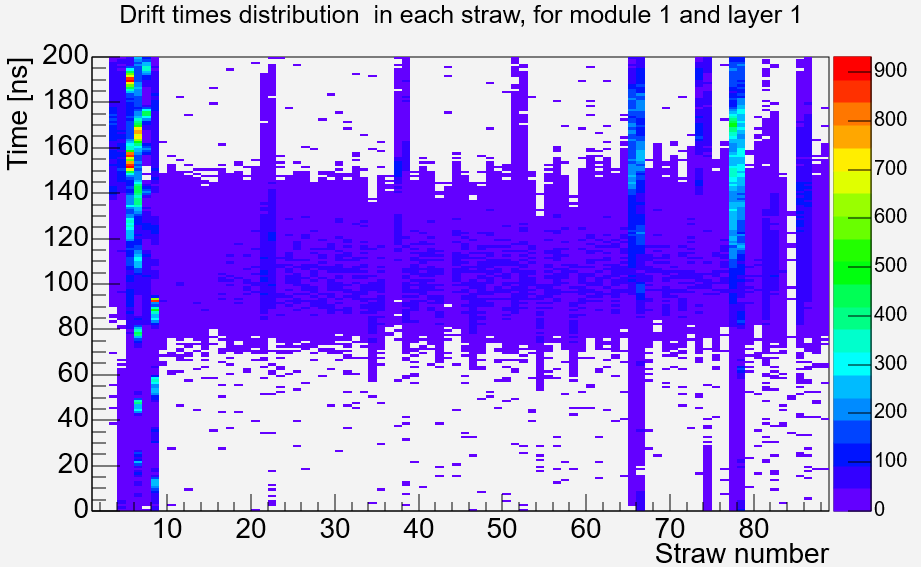
\includegraphics[width=0.47\columnwidth]{uncalib_drift2d_m1l1.png}}}
	\quad
	\centering
	\subfloat[Module 1, Layer 1 (Calibrated) \label{subfig:drift2d_layer_m1l1c}]{{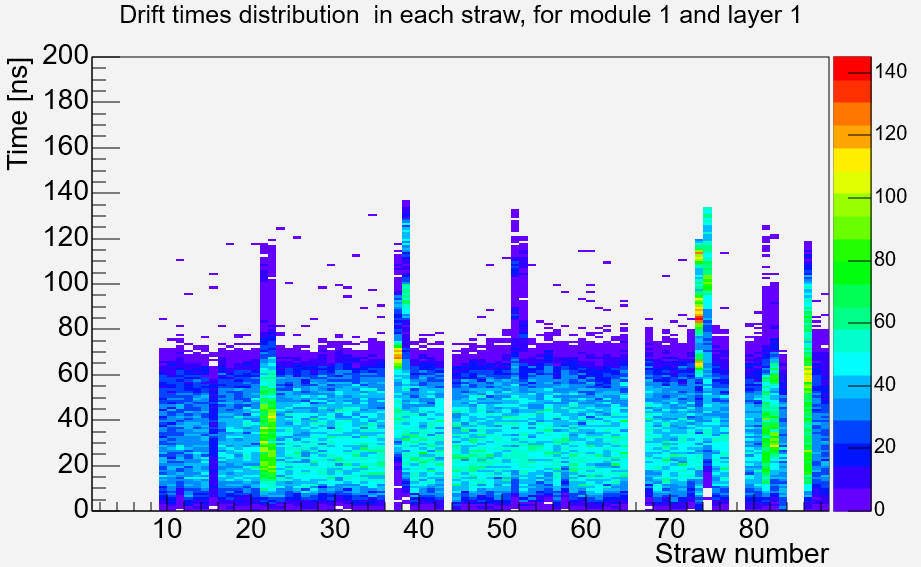
\includegraphics[width=0.47\columnwidth]{calib_drift2d_m1l1.png}}}
	\quad
	\centering
	\subfloat[Module 3, Layer 1 (Uncalibrated) \label{subfig:drift2d_layer_m3l1uc}]{{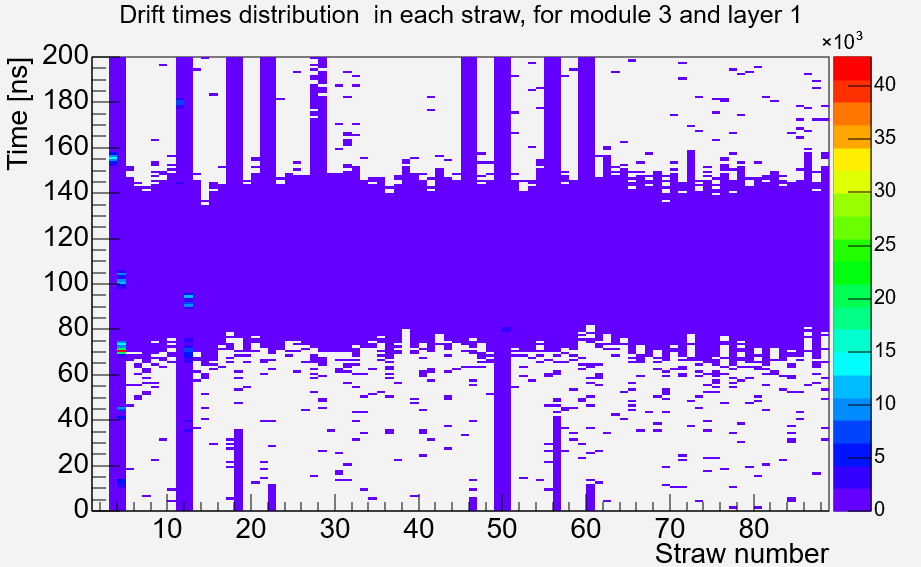
\includegraphics[width=0.47\columnwidth]{uncalib_drift2d_m3l1.png}}}
	\quad
	\centering
	\subfloat[Module 3, Layer 1 (Calibrated) \label{subfig:drift2d_layer_m3l1c}]{{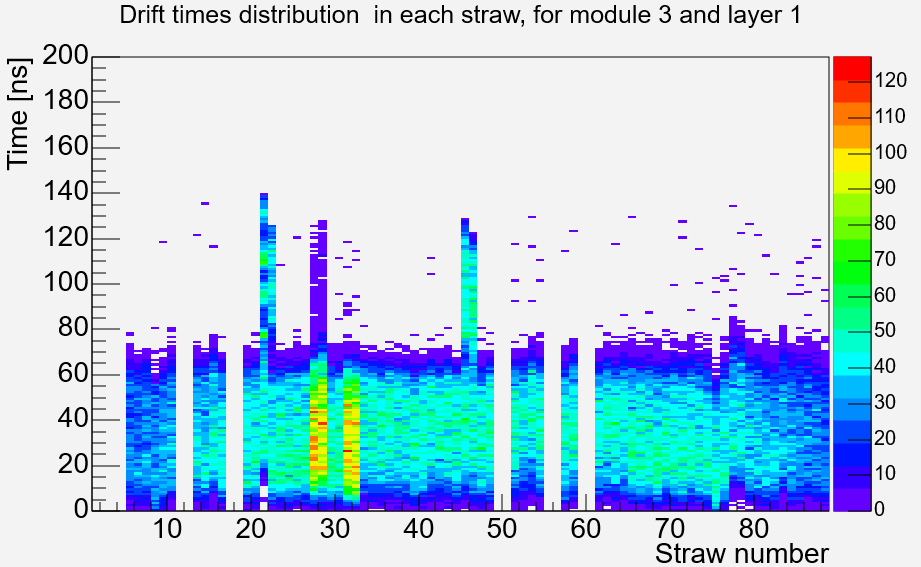
\includegraphics[width=0.47\columnwidth]{calib_drift2d_m3l1.png}}}
	\caption{The uncalibrated (left) and calibrated (right) 2-D drift time 
	distributions for different layers and modules of the apparatus. The number of entries for each straw at each time is shown in the 
	color axis.}
	\label{fig:calib_drift2d_layer}
\end{figure*}

As with the 1-D drift time distributions, we observe that the calibration has been correctly implemented. We observe that while the 
uncalibrated distributions have uneven starting times for each straw (observed by the non-uniformity of the histogram), the calibrated 
distributions both start from $\SI{0}{\nano\second}$. Additionally, the fluctuations in the distribution caused by the noise
in the data is filtered out in the calibrated distribution as the majority of the signal is observed within $20 - 60 \si{\nano\second}$. 
This is especially evident for the distribution with Module 3, Layer 1 (Fig. \ref{subfig:drift2d_layer_m3l1uc} and \ref{subfig:drift2d_layer_m3l1c}). 
While the signal is dominated by background in the uncalibrated data, the signal is apparent once the calibration is applied. \par 

We also observe that the dead straws have been removed after calibration. In Fig. \ref{subfig:drift2d_layer_m1l1c}, we observe that 
straws 37, 43, 66, 78, and 85, as well as all straws from 1 - 9 have been removed in the distribution. The reason for this is clear as we see that 
the drift time measured by most of these straws extend past the observed drift time distribution from the other straws (as shown in Fig. 
\ref{subfig:drift2d_layer_m1l1uc}), indicating that the distribution does not fit the desired shape. See Appendix (Chap. \ref{chap:appendix}) for the drift time 
distribution for some of these particular straws. \par 

The calibration program also shows a strawmap that displays the status of each straw in our detector. The calibration program 
identifies each straw as either OK (green), HOT (blue), dead (red), or continuous (yellow) based on the drift time distribution 
for each straw. Straws that are either HOT or dead indicate that there is some problem with the front-end chip of the straw.
Fig. \ref{fig:calib_strawmap} shows the strawmap for the detector used in our experiment. 

\begin{figure*}[!h]
	\centering
	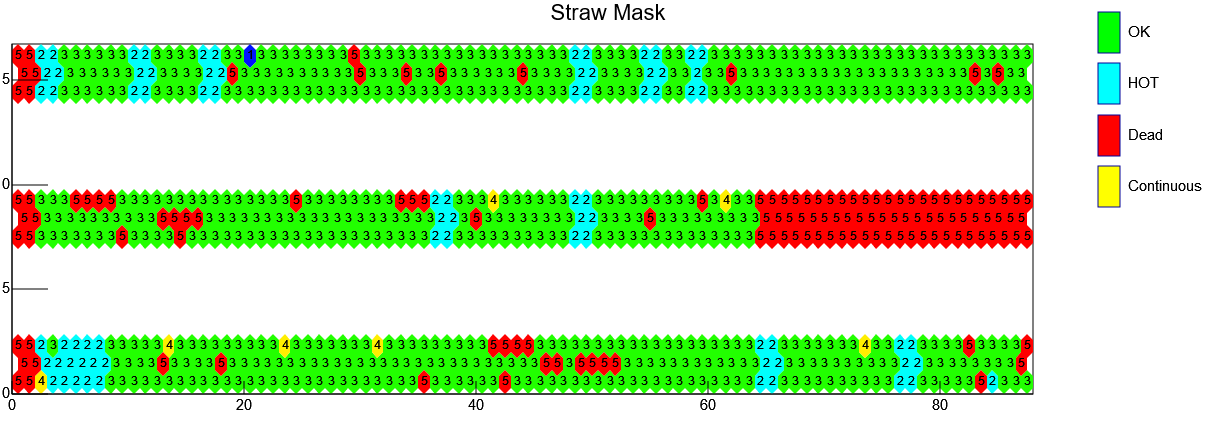
\includegraphics[width=0.8\textwidth]{calib_strawmask.png}
	\caption{The straw map of the detector used in this experiment. The status of each straw is marked as OK (green, 3), 
	HOT (blue, 2), dead (red, 5), and continous (yellow, 4). The modules and layers are presented from lowest 
	(Module 1, Layer 1) to highest (Module 3, Layer 3).}
	\label{fig:calib_strawmap}
\end{figure*}

From the bottom of the strawmap (corresponding to Module 1), we observe that the same straws that showed problematic drift time distributions
in Fig. \ref{subfig:drift2d_layer_m1l1uc} (straws 1 - 9, 37, 43, 66, 78, 85) are indicated as either HOT or Dead. Furthermore, 
we observe that in Module 2, straws 66 and higher are dead straws. This is also reflected in the calibrated drift time distribution 
for Layers in Module 2 (see Appendix (Chap. \ref{chap:appendix})). \par 

\chapter{Analysis} \label{chap:track_analysis}

In this chapter, we use the straw-by-straw calibration method as discussed in Sec. \ref{sec:straw_calib} onto the 
raw data taken overnight to reconstruct the events to obtain the tracks deposited by the cosmic ray muons. 
We then analyze the distributions obtained from these reconstructed tracks. \par 

\section{Procedure} \label{sec:analysis_proced}

We first ran the \texttt{StyxM2C2} program as with the calibration step. As we have used the first 300 000 events for 
calibration purposes, we skipped these events and ran the program for the subsequent 200 000 events. The calibration 
performed in Chap. \ref{chap:calib} was applied by providing the output calibration file in the argument. 
All in all, we ran the following command for this processing procedure: 
\begin{tcolorbox}
	\begin{verbatim}
		StyxM2C2 -S 300000 -N 200000 -C CalibM2C2300k.txt -O TrackingM2C2200k.txt
			 -I ../te22132161802.hld --no-clean --all
	\end{verbatim}
\end{tcolorbox}

We then used the \texttt{StyxLabCourse} program to reconstruct the events to obtain the muon tracks. This program controls the 
bulk event generation, reconstruction, and finally analyzes the reconstructed tracks as 1-D or 2-D histograms. 
The output is returned as a ROOT file and can be plotted using ROOT \cite{labman}. The two most relevant codes in which we had 
to modify in this program is \texttt{StudentAnalysis.cxx}, which constructs and fills the histograms with parameters of interest,
and \texttt{labCourse.cpp}, which contains the main function that runs the reconstruction and analysis from the provided 
calibration and data file. \par 

\section{Results: Hits per Straws}

We first constructed histograms for the number of hits per straw for each layer. Fig. \ref{fig:hitsperstraw_m1_layers} shows the number of hits per straw for 
Module 1 for each layer. We observe that generally the number of hits are higher for straws 30 - 60 (located in the inner region of the 
detector) compared to the other straws (located in the edges of the detector). 
This is due to the geometry of the detector. As the detector has a trapezoidal structure and since the scintillator only covers
the inner straws, the events detected from the outer straws are not triggered, thus yielding less hits. We also observe that there are 
some regions in which there are no counts, which are associated to the dead straws that are removed from the calibration as shown in 
Fig. \ref{fig:calib_strawmap}. \par 

When comparing between the layers, we observe no major differences between the distributions. Furthermore, the peaks observed 
in each distribution occur at approximately the same location, indicating that such peaks are not due to background or noise. 
\textcolor{red}{explain the peak or nah?} \par 


\begin{figure*}[htb!]
	\centering
	\subfloat[Layer 1]{{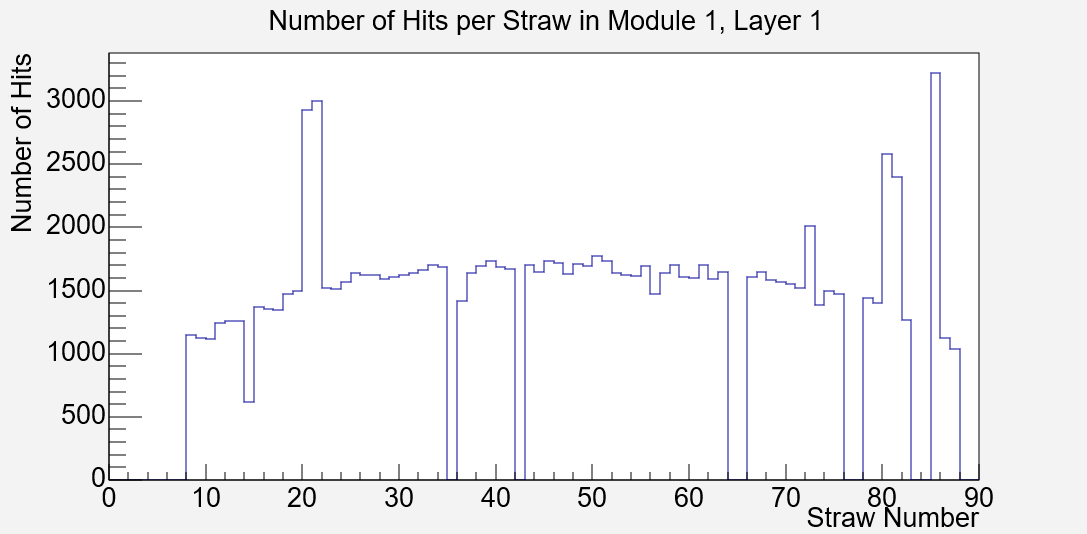
\includegraphics[width=0.47\columnwidth]{hitsperstraw_m1l1.png}}}
	\quad
	\centering
	\subfloat[Layer 2]{{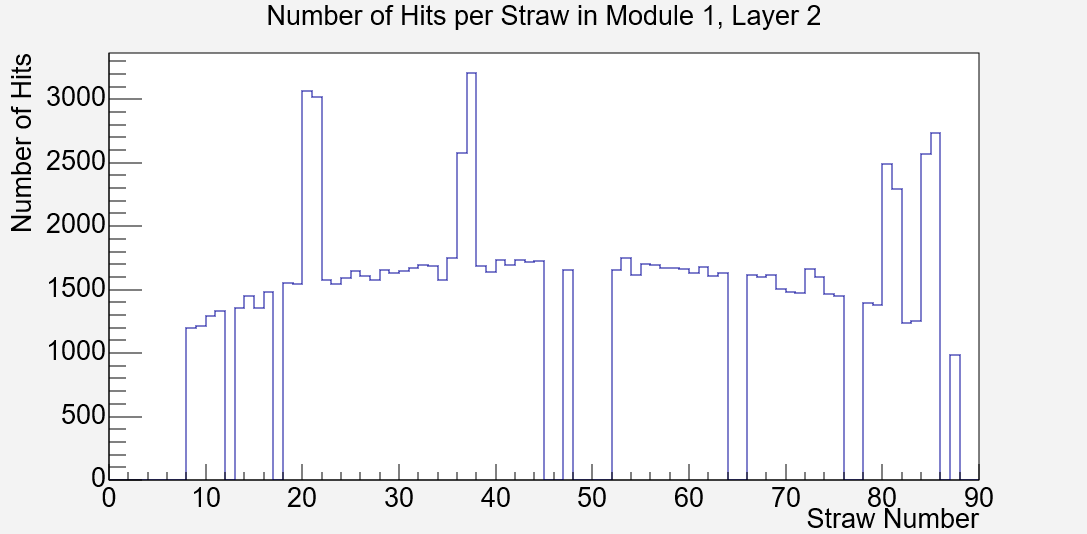
\includegraphics[width=0.47\columnwidth]{hitsperstraw_m1l2.png}}}
	\quad
	\centering
	\subfloat[Layer 3]{{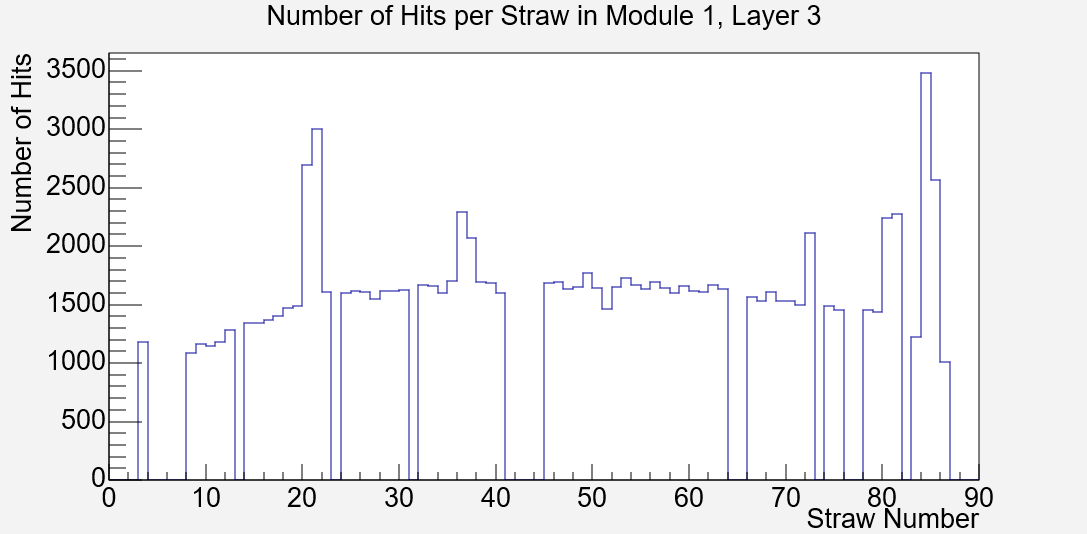
\includegraphics[width=0.47\columnwidth]{hitsperstraw_m1l3.png}}}
	\caption{The number of hits per straw at each layer of module 1. }
	\label{fig:hitsperstraw_m1_layers}
\end{figure*}

We also constructed histograms for the number of hits per straw for all layers for each module. Fig. \ref{fig:hitsperstraw_modules} shows this distribution for 
each module (module 1 - 3). We observe that the general structure of the distribution is similar to that of the distribution for 
each layer (Fig. \ref{fig:hitsperstraw_m1_layers}). We also observe the same dead straws as observed in the strawmap in Fig. \ref{fig:calib_strawmap}.


\begin{figure*}[htb!]
	\centering
	\subfloat[Layer 1]{{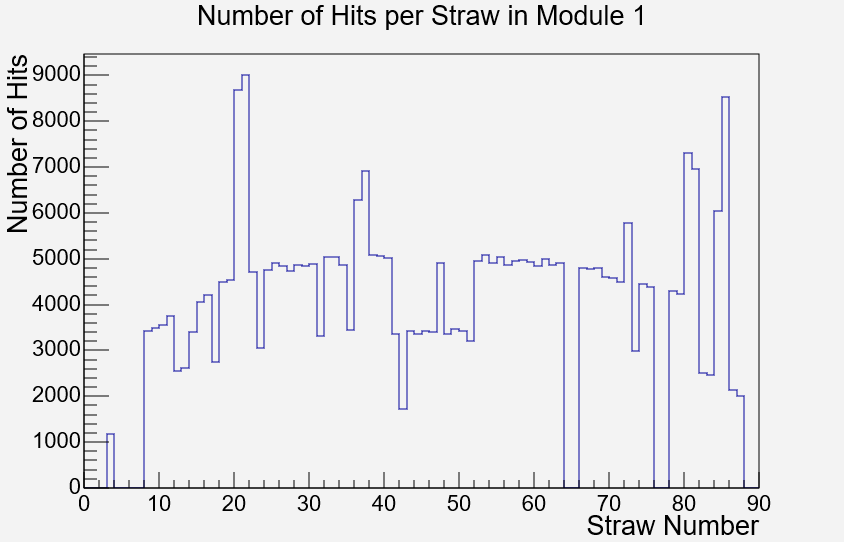
\includegraphics[width=0.47\columnwidth]{hitsperstraw_m1.png}}}
	\quad
	\centering
	\subfloat[Layer 2]{{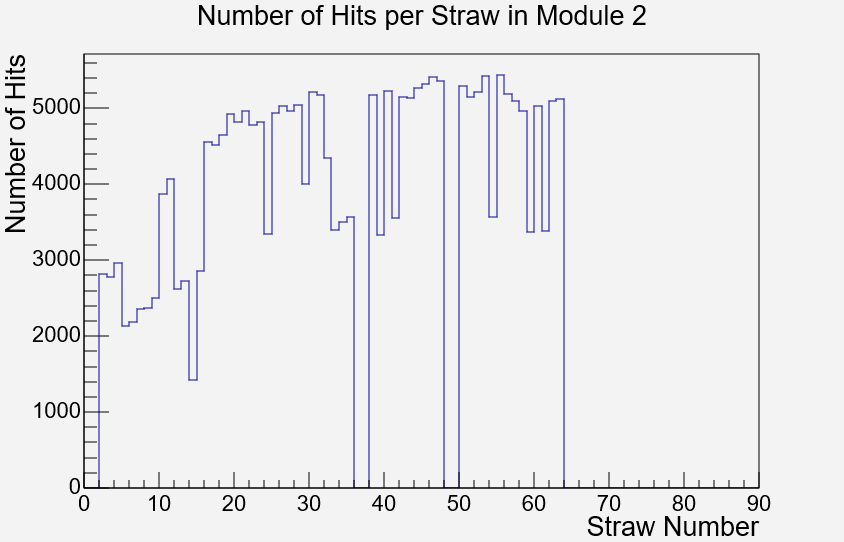
\includegraphics[width=0.47\columnwidth]{hitsperstraw_m2.png}}}
	\quad
	\centering
	\subfloat[Layer 3]{{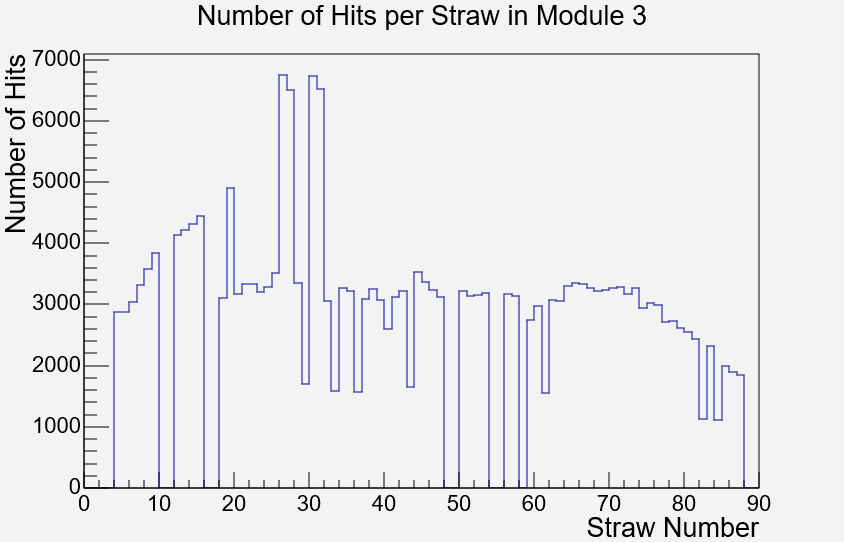
\includegraphics[width=0.47\columnwidth]{hitsperstraw_m3.png}}}
	\caption{The number of hits per straw for each module by taking into account the hits per straw for each layer. }
	\label{fig:hitsperstraw_modules}
\end{figure*}

We also compare between the hits per straw from module 1 and module 3, shown in Fig. \ref{fig:tracksvshits_comp}. From this, we observe that the shape of the 
distribution is the same for both modules, however the amplitude is decreased by approximately 2000 entries from straw 20 onwards. 

\begin{figure*}[!h]
	\centering
	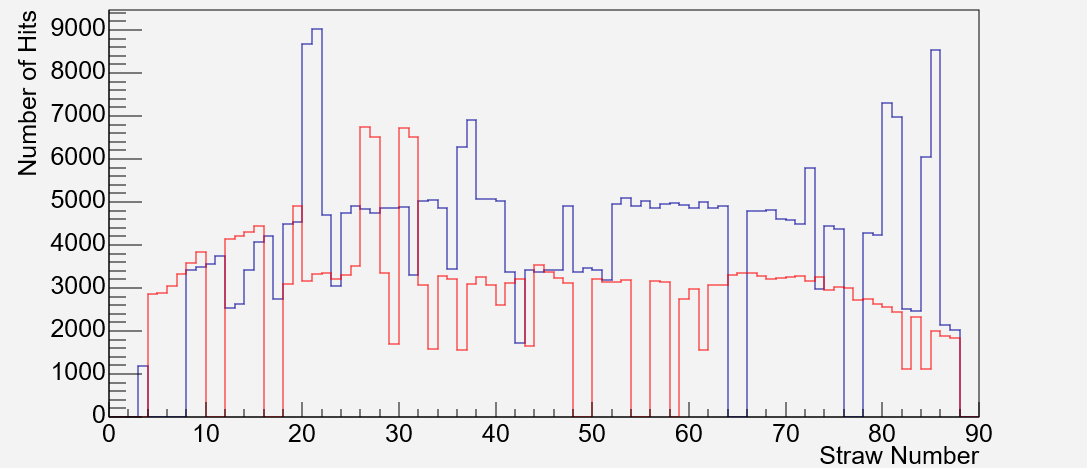
\includegraphics[width=0.8\textwidth]{hitsperstraw_m1m3.png}
	\caption{Comparison of number of hits per straw between module 1 (blue) and 3 (red). }
	\label{fig:tracksvshits_comp}
\end{figure*}

\section{Results: Tracks}

We now plot the two-dimensional histogram between the number of tracks and the number of hits per event in the detector. Fig. \ref{fig:tracksvshits}
shows this two-dimensional histogram. From this, we observe that we need approximately 8 hits per event to construct 1 track per event
as the peak of the histogram is located at this point. This is consistent with the distribution of the number of hits triggered in 
the detector (see Appendix (Chap. \ref{chap:appendix})).  \textcolor{red}{not too sure about this part: }Furthermore, we observe that the distribution is strongly peaked, implying that 
the reconstruction algorithm mainly constructs one or two tracks at most. \par 

\begin{figure*}[!h]
	\centering
	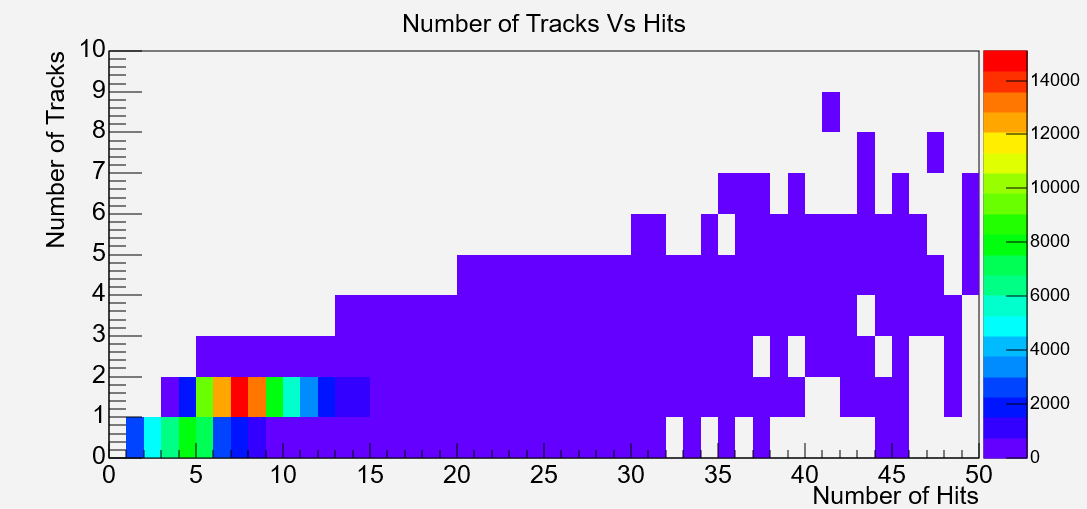
\includegraphics[width=0.8\textwidth]{trackvshits.png}
	\caption{The two-dimensional histogram between the number of hits and the number of tracks per event. 
			The color axis represents the number of entries for each track and hits per event.}
	\label{fig:tracksvshits}
\end{figure*}

We also show the angular distribution of all tracks obtained from the reconstruction in Fig. \ref{fig:tracksangle}. To obtain this distribution, we 
plot the number of tracks against the slope of the muon tracks. The angle is then obtained via the following equation:
\begin{equation}
	m = \tan \theta
\end{equation}
where $\theta$ is the incoming angle of the track, so that an angle of $\SI{0}{\degree}$ corresponds to a particle that enters the 
detector in a perpendicular fashion. From observing the shape of the distribution, we observe that the number of tracks, that is, 
the number of particles, decreases as one moves further from the local zenith as expected. This is due to the fact that a muon with a 
higher incoming angle interacts more with the atmosphere, thus increasing the probability that it will be stopped by the atmospheric
particles. \par 

\begin{figure*}[!h]
	\centering
	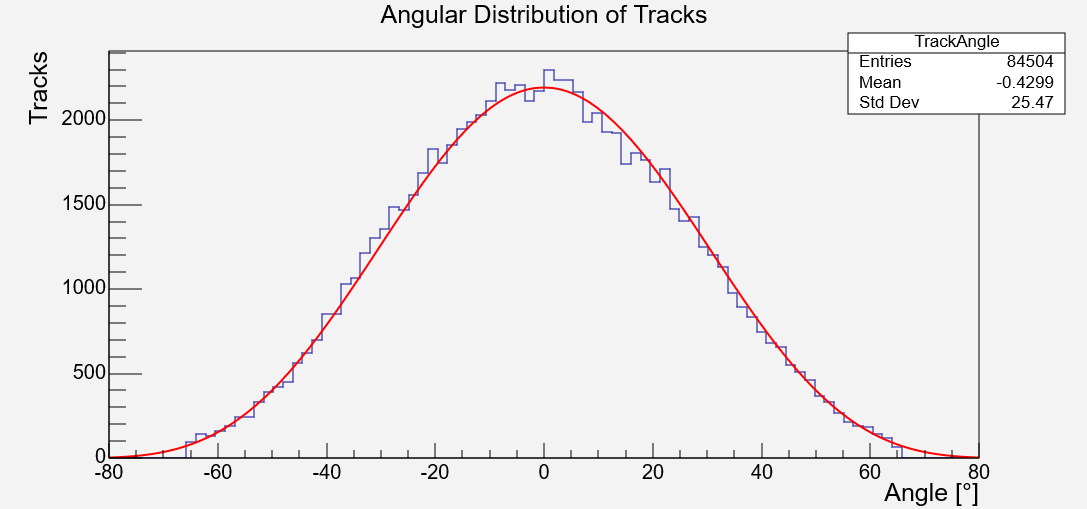
\includegraphics[width=0.8\textwidth]{trackangle.png}
	\caption{The angular distribution of the reconstructed tracks. The red line indicates the fit function $I = I_0 \cos^n \theta$
			to the data. }
	\label{fig:tracksangle}
\end{figure*}


We further fit the distribution by the intensity distribution given in Eq. \ref{eq:muon_intensity}. From using the fitting 
program provided by ROOT, we obtain that $I_0 = \num{2193.7 \pm 9.5}$ \textcolor{red}{units} and $n = \num{3.846 \pm 0.024}$. This implies that 
the intensity distribution that we have obtained does not follow the intensity distribution of muons at sea level ($n = 2$). 
An attempt to fit a function $\propto \cos ^2 \theta$ is shown in Fig \ref{fig:tracksangle_cos2fit}. 

\begin{figure*}[!h]
	\centering
	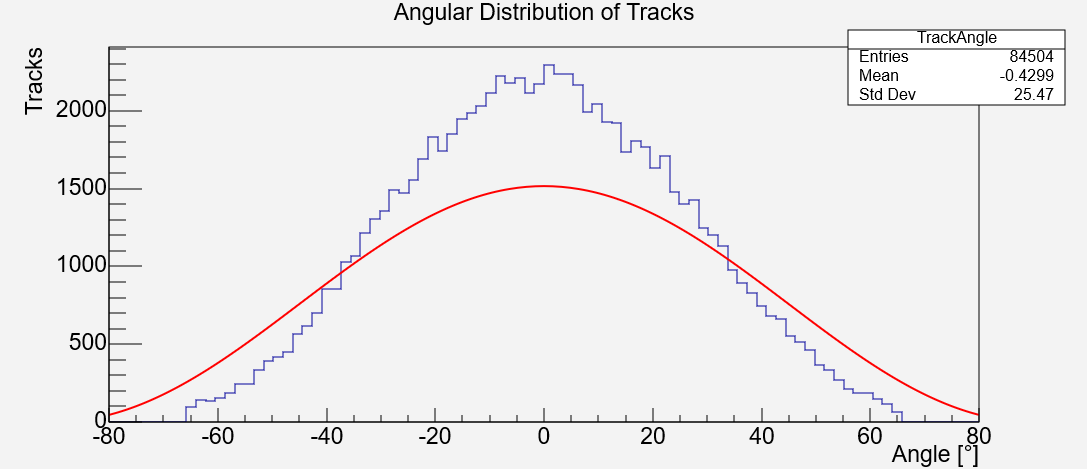
\includegraphics[width=0.8\textwidth]{trackangle_cos2fit.png}
	\caption{Same as Fig. \ref{fig:tracksangle} but for the fit function $I = I_0 \cos^2 \theta$ (red line) instead. }
	\label{fig:tracksangle_cos2fit}
\end{figure*}

% The deviation from our results to the expected results can be caused by the geometry of the detector. As mentioned in previous
% sections, the scintillators are only located in the inner region of the trapezoidal detector, and as such the 

Finally, we compare our reconstructed tracks with the segment for events with only one track. 
The segment is the tangent line between two or more circles with radii between the anode and the measured position of the straw. 
Fig. \ref{fig:trackvssegment} shows the two-dimensional histogram between the track and segment angle. \textcolor{red}{need to add interpretation of results}.

\begin{figure*}[!h]
	\centering
	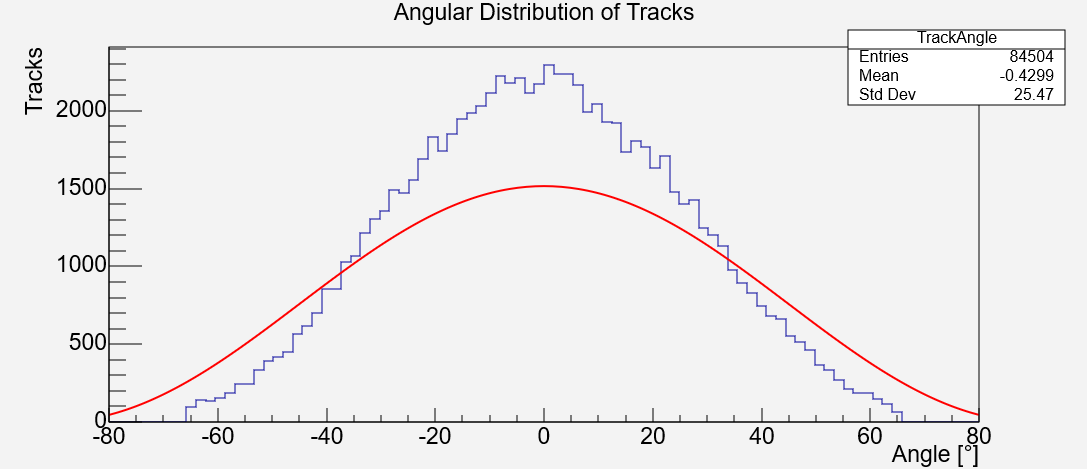
\includegraphics[width=0.8\textwidth]{trackangle_cos2fit.png}
	\caption{The histogram between the track angles and segment angles for events with only one track. The 
	color axis represents the number of entries per track and segment angle. }
	\label{fig:trackvssegment}
\end{figure*}

\chapter{Conclusion} \label{chap:concl}

In this report, we determined the intensity distributions from secondary cosmic ray muons using a drift chamber detector. 
The detector was constructed by three modules, each with 88 straws and 3 layers each, with scintillators placed in between them. \par 

We first set up the trigger system to determine the optimal voltage by varying the voltage of the lower photomultiplier tube (PMT) 
until we observe a linear behaviour in the distribution. The optimal voltage was set to be the initial point in which the line begins, and
in our experiment this was set to be 2100V. We then modified the upper voltage of the PMT by looking at the coincidence rate between the 
upper and lower PMT. The optimal upper voltage was chosen to be 2000V, which is where the plateau of the distribution begins. \par 

We then determine the front-end threshhold voltage, i.e. the optimal voltage for the front-end boards in the apparatus. 
The optimal voltage was chosen by varying the voltage and choosing the histogram between time and number of hits 
which yields the lowest noise and the highest count. In our experiment, we obtained the front-end threshhold voltage to be 
2V. An overnight measurement was then taken using these voltage settings.\par 

We then calibrated the data using the straw-by-straw calibration method which corrects the offsets in the drift time distribution
for each straw. We also removed the dead straws that showed problematic distributions when observing their drift time distributions. 
From the obtained figures, we were successfully able to calibration our obtained overnight data. \par 

Finally, we used the constructed calibration file to reconstruct the number of muon tracks. The number of hits per straw generally 
had the same behaviour which was attributed to the geometry of the apparatus. No clear differences were observed between each layer 
of a module, but there was a decrease in the amplitude when comparing between module 1 and module 3. \par 

We then observed the histograms from the reconstructed tracks. We observed from the distribution between number of hits and tracks 
that we need approximately $\sim 8$ hits to construct one track per event. The angular distribution yielded a fit value of 
$I_0 = \num{2193.7 \pm 9.5}$ \textcolor{red}{units} and $n = \num{3.846 \pm 0.024}$, which deviates from the expected behaviour of 
$\cos^2 \theta$. \textcolor{red}{add things about track vs segment angle.}

In the end, we were successfully able to measure the muon distribution from cosmic rays at sea level. However, we did not obtain
the expected behaviour of the distribution. \textcolor{red}{add future ideas}


\chapter{Acknowledgements}

\printbibliography

\chapter{Appendix} \label{chap:appendix}

In this section, we show additional plots that are of interest to our report.\par 

\begin{figure*}[htb!]
	\centering
	\subfloat[Straw 7]{{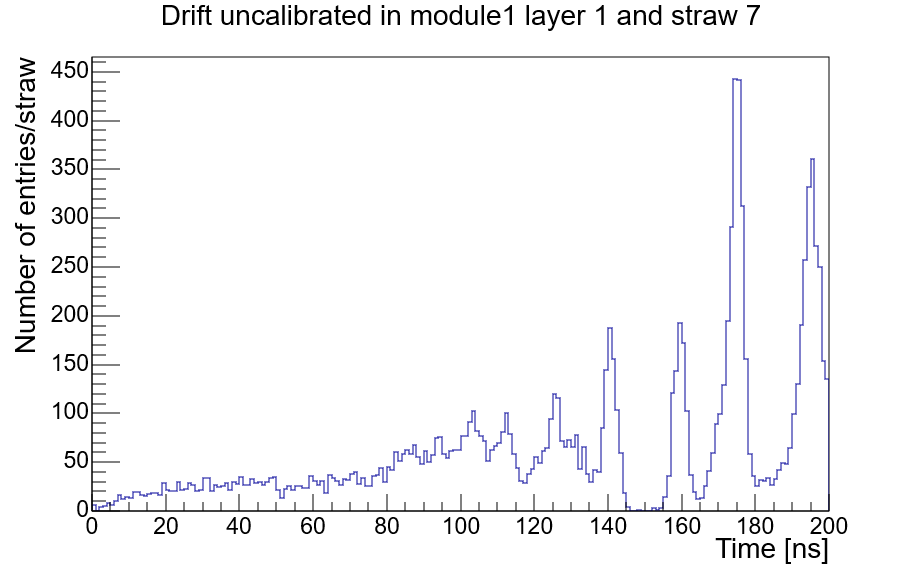
\includegraphics[width=0.47\columnwidth]{uncalib_drift_m1l1s7.png}}}
	\quad
	\centering
	\subfloat[Straw 37]{{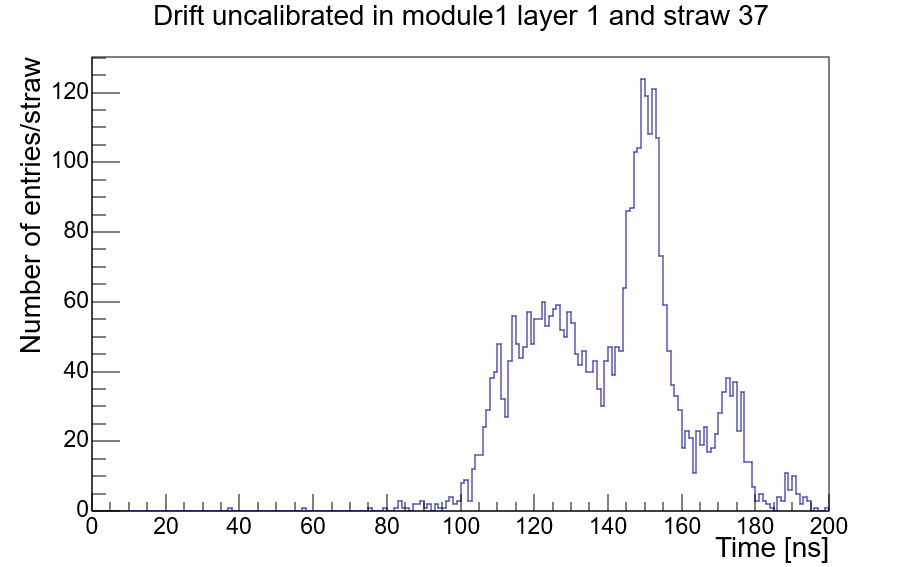
\includegraphics[width=0.47\columnwidth]{uncalib_drift_m1l1s37.png}}}
	\quad
	\centering
	\subfloat[Straw 66]{{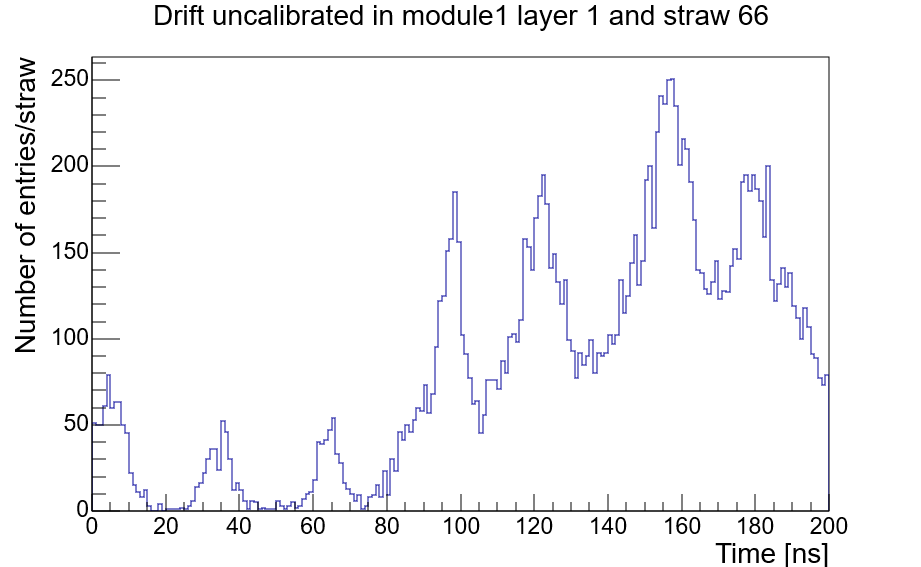
\includegraphics[width=0.47\columnwidth]{uncalib_drift_m1l1s66.png}}}
	\quad
	\centering
	\subfloat[Straw 78]{{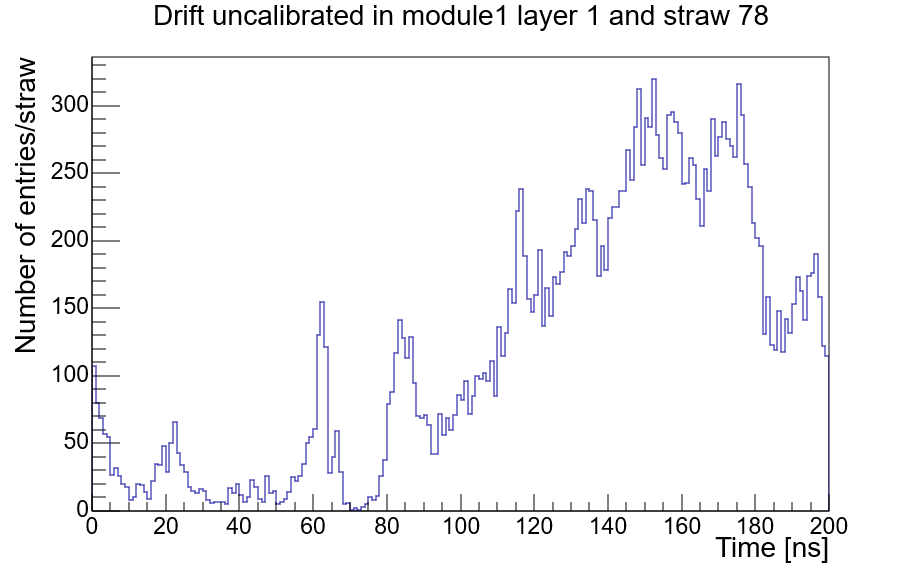
\includegraphics[width=0.47\columnwidth]{uncalib_drift_m1l1s78.png}}}
	\caption{The uncalibrated drift time distributions for Module 1, Layer 1 for straws that have been removed 
	in the calibration process.}
	\label{fig:calib_drift_straws}
\end{figure*}

\begin{figure*}[htb!]
	\centering
	\subfloat[Uncalibrated]{{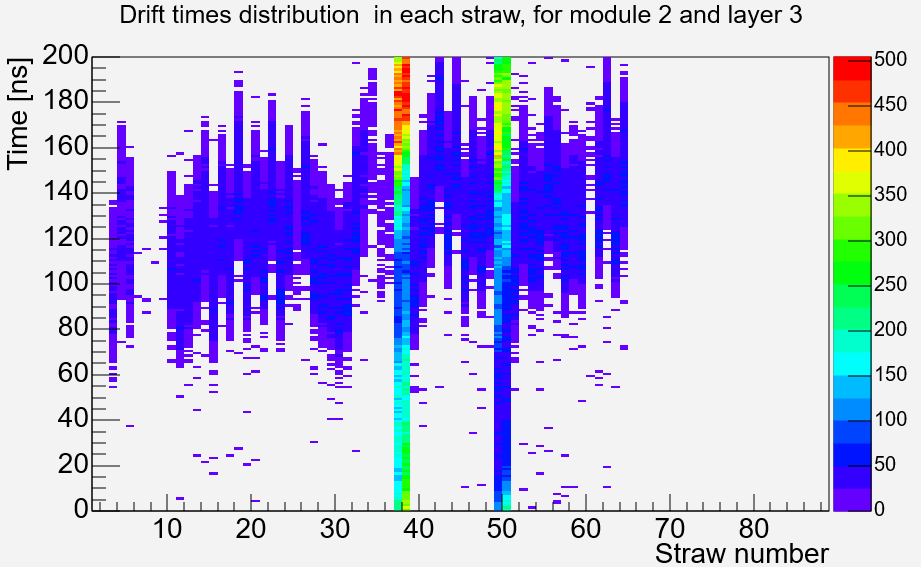
\includegraphics[width=0.47\columnwidth]{uncalib_drift2d_m2l3.png}}}
	\quad
	\centering
	\subfloat[Calibrated]{{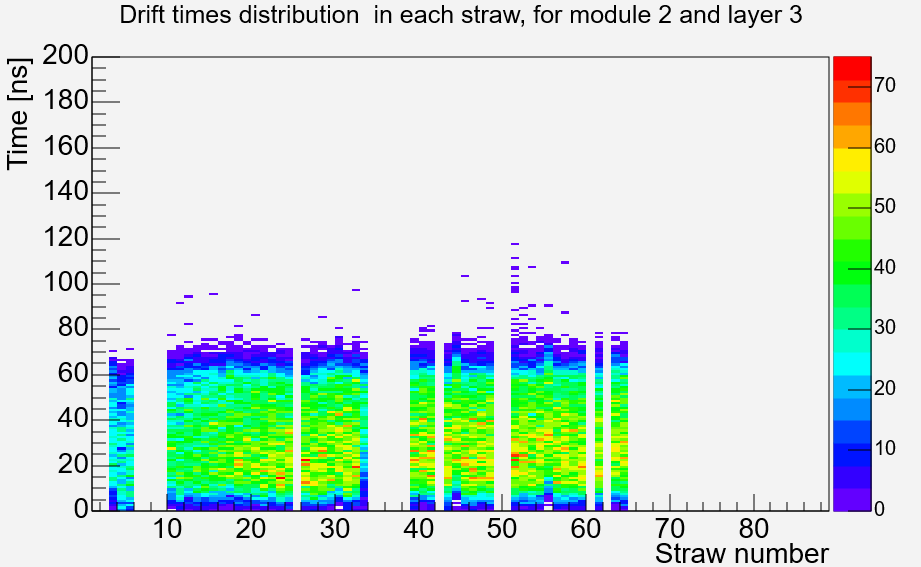
\includegraphics[width=0.47\columnwidth]{calib_drift2d_m2l3.png}}}
	\caption{The uncalibrated and calibrated 2-D drift time 
	distributions for Module 2, Layer 3. The number of entries for each straw at each time is shown in the 
	color axis.}
	\label{fig:calib_drift2d_m2l3}
\end{figure*}

\end{document}


